\section{Rethinking storage for Docker registry}
\label{sec:file_adressable}
%\vcomment{Nannan, please, do not use lines longer than 80 characters. It will simplify review
%and revision process.}\nancomment{Addressed}
%\nancomment{Converted to discussion}
%
%\subsection{}
%\paragraph{Benefit of file-level content addressable storage}
%
%Currently, Docker registry uses layer-level content addressable storage model
%to avoid storing redundant copies of an identical layer.  However, as discussed
%in previous sections, almost 97\% of files inside the layers are redundant
%which accounts for 86\% of storage space (uncompressed).  
As the number of images stored in Docker registry is increasing dramatically,
storing and managing the large proportion of redundant files requires both
storage equipment and administration investment. 
%
In this section, as an
alternative to layer-level content addressable storage, a file-level content
addressable storage model (FLCAS) is suggested for Docker registry to remove
redundant files.% and save space while maintaing good performance.

FLCAS, which is essentially a file-level deduplication, can significantly
reduce the redundant files in docker registry and save a large volume of
storage space. 
%
However, FLCAS may also introduce considerable overheads, which
include decompressing compressed layer archival files, calculating the file
content digest, searching for identical files, etc.  
%
To reduce above overhead,
we provide different suggestions on how one can mitigate the affects of such
overheads and efficiently server push/pull requests. 
%
We also simulated FLCAS on
0.9 million layers and provided performance analysis.

%\lrcomment{These challenges should be listed earlier in the section. They are
%also hard to follow as at this point, it it is still unclear why we need
%searching or why we have additional compression/decompression overhead.} while
%maintain a good performance. 
%\lrcomment{What are the challenges we overcome with FLCAS?}  
%Docker registry can save a lot of space if using file-level content addressable storage. 
%Benefit: saving money, reducing storage management overhead.

\subsection{File-level content addressable storage model (FLCAS)}
File-level content addressable storage system (FLCAS) uses file-level
deduplication to remove the redundant copies of an identical file by generating
a digest (such as MD5 or SHA256) from the file the digest refers to.
%
Consequently, FLCAS exposes a high-level layer addressing by mapping layer
digests to their containing file digests. 

File-level deduplication mainly consists of three
steps: layer decompression, file content digest calculation, and searching \&.
indexing. 
% 
During file-level deduplication, the unique files are stored in a
\textit{file pool} and redundant copies are removed. 
%
A unique \textit{file
content address} is recorded, which is a file digest uniquely and linked to the
files'location. 
%
Meanwhile, a layer digest to its containing file content digest
mapping record is also created and saved to a \textit{layer-to-file digest
table}.     

\paragraph{Deduplicating when workload is light}

\begin{figure}[t]
	\centering
		\begin{minipage}{0.24\textwidth}
			\centering
			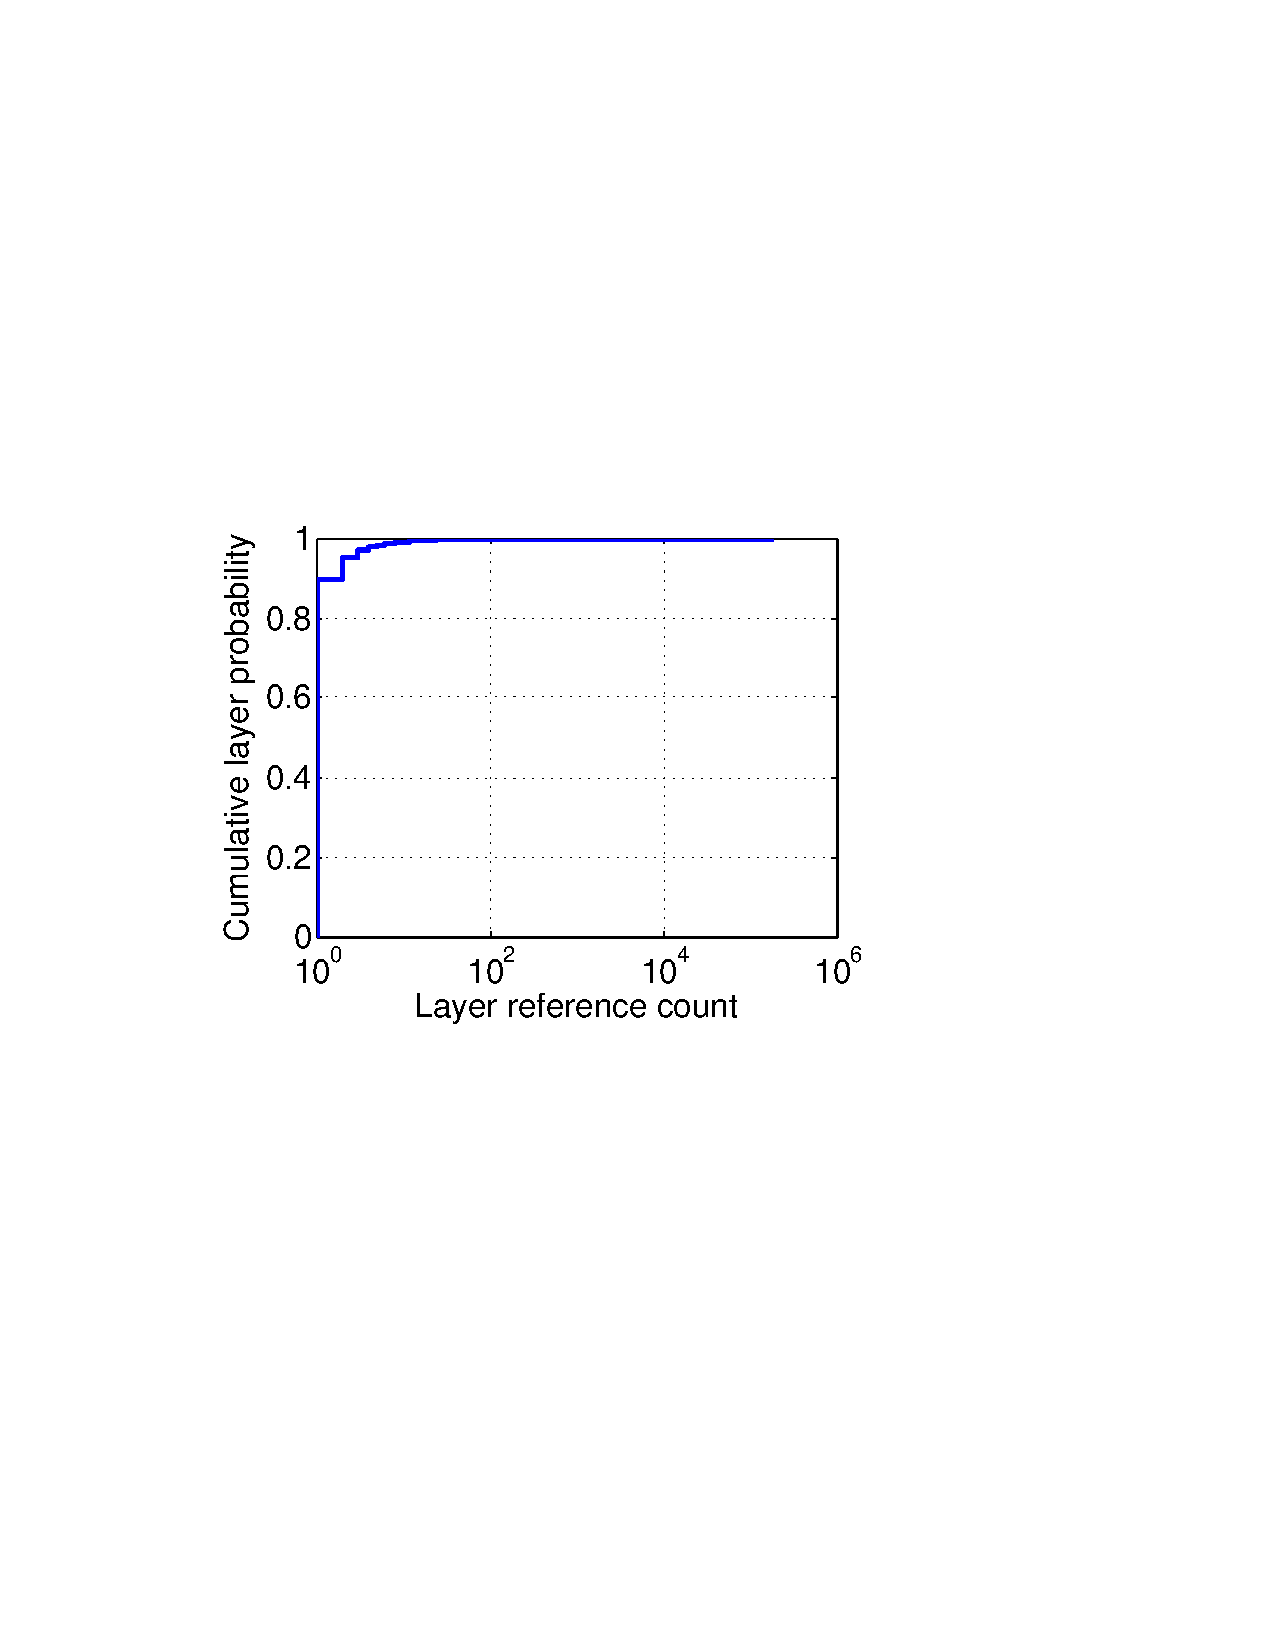
\includegraphics[width=1\textwidth]{graphs/shared-cnt-cdf.pdf}
			\caption{CDF of layer\\\ reference count.}
			\label{fig:ref_count}
		\end{minipage}
	\begin{minipage}{0.22\textwidth}
		\centering
		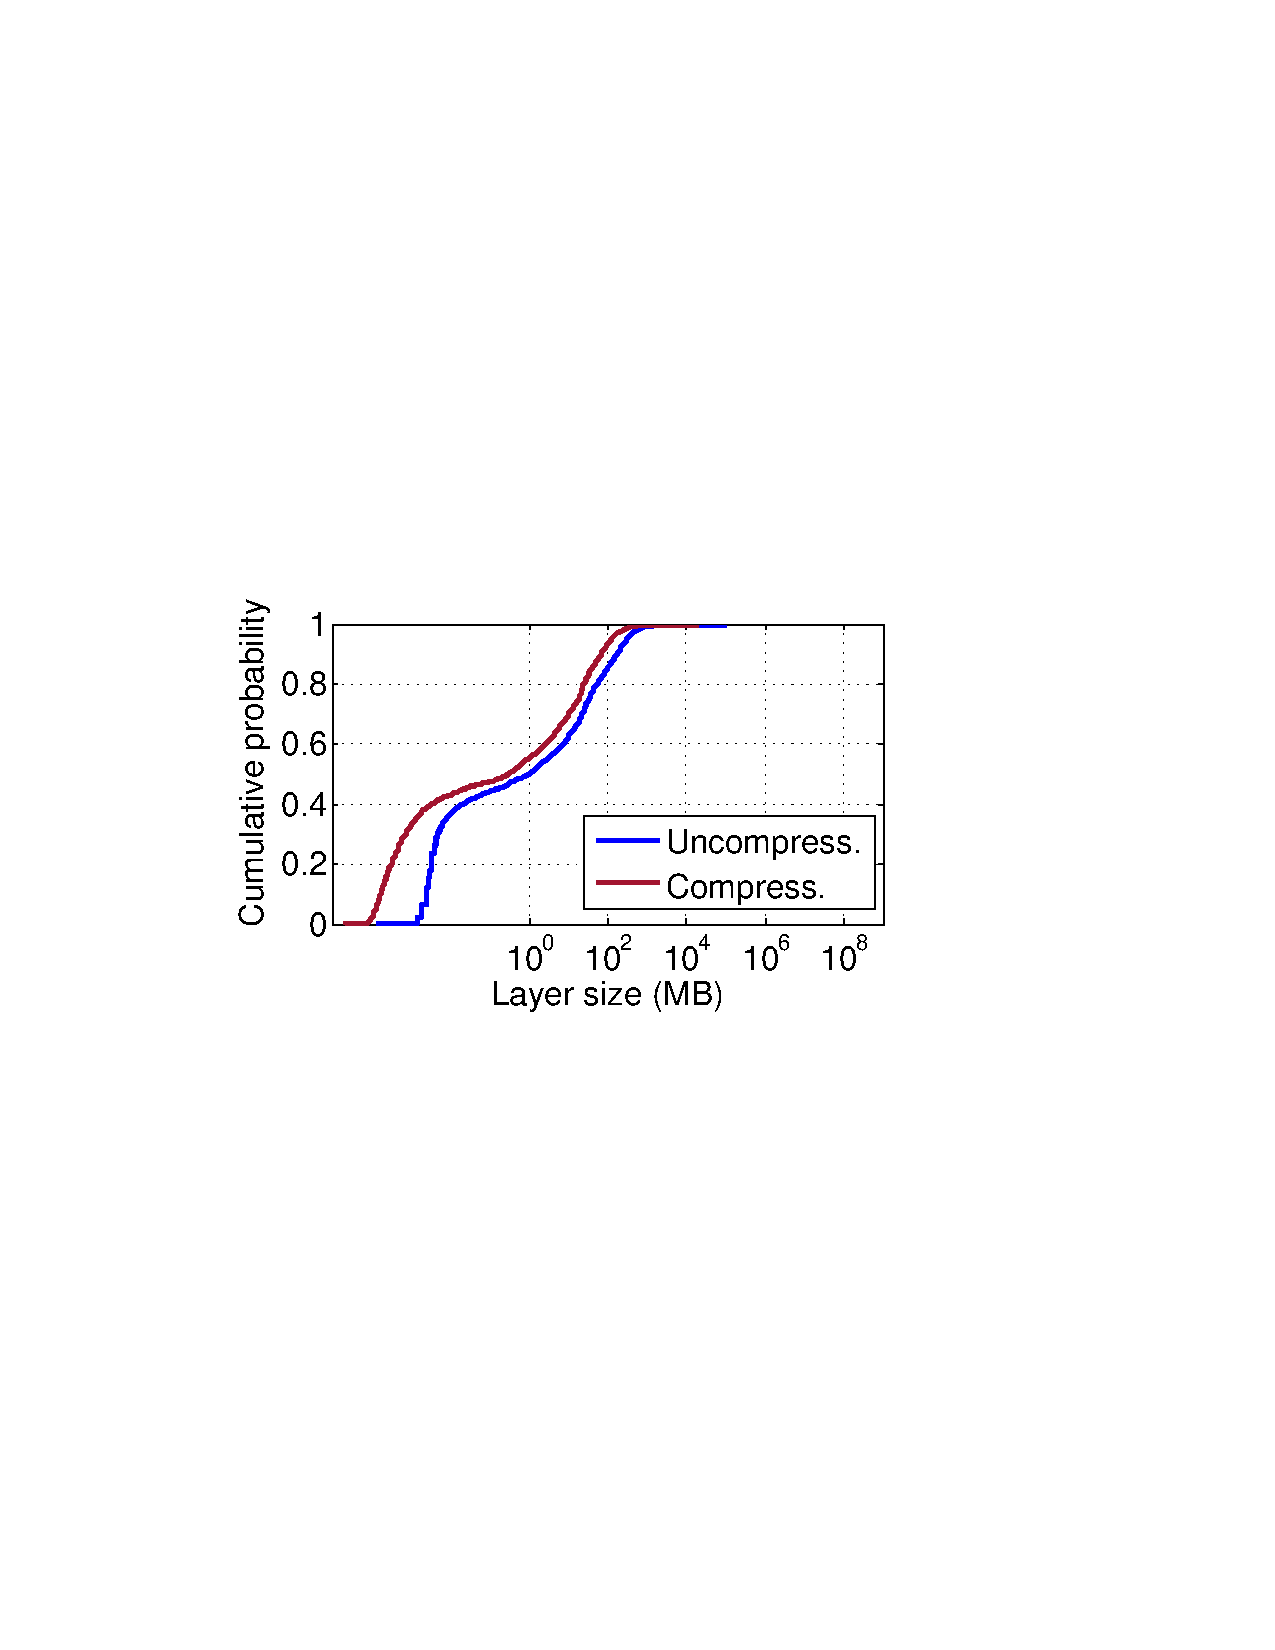
\includegraphics[width=1\textwidth]{graphs/layer-size-cdf.pdf}
		\caption{CDF of compress. and uncompress. layer size.}
		\label{fig:layer-size-cdf}
	\end{minipage}
\end{figure}


Deduplication can be expensive in terms of performance overhead, file-level
dedupilication can be triggered for removing the redundant files for cold
layers only when the workload is low and storage utilization is high.
%  
Typically,
workload fluctuates, with peaks and troughs. 
%
According to IBM container
registry workload analysis~\cite{dockerworkload}, 80\% of time, there were only 100
requests.
%
To improve performance, we also suggest to use
RAM to temporarily store \textit{small} layers and directly process them in RAM
to perform decompression, unpacking, file content digest calculation.
%
According to our findings majority (87.3\%) of layers that are less than 50M as
shown in Figure~\ref{fig:layer-size-cdf}.
%
So majority of layers can be stored
and processed in RAM to speed up file-level dedup. 

\begin{figure}
	\centering
	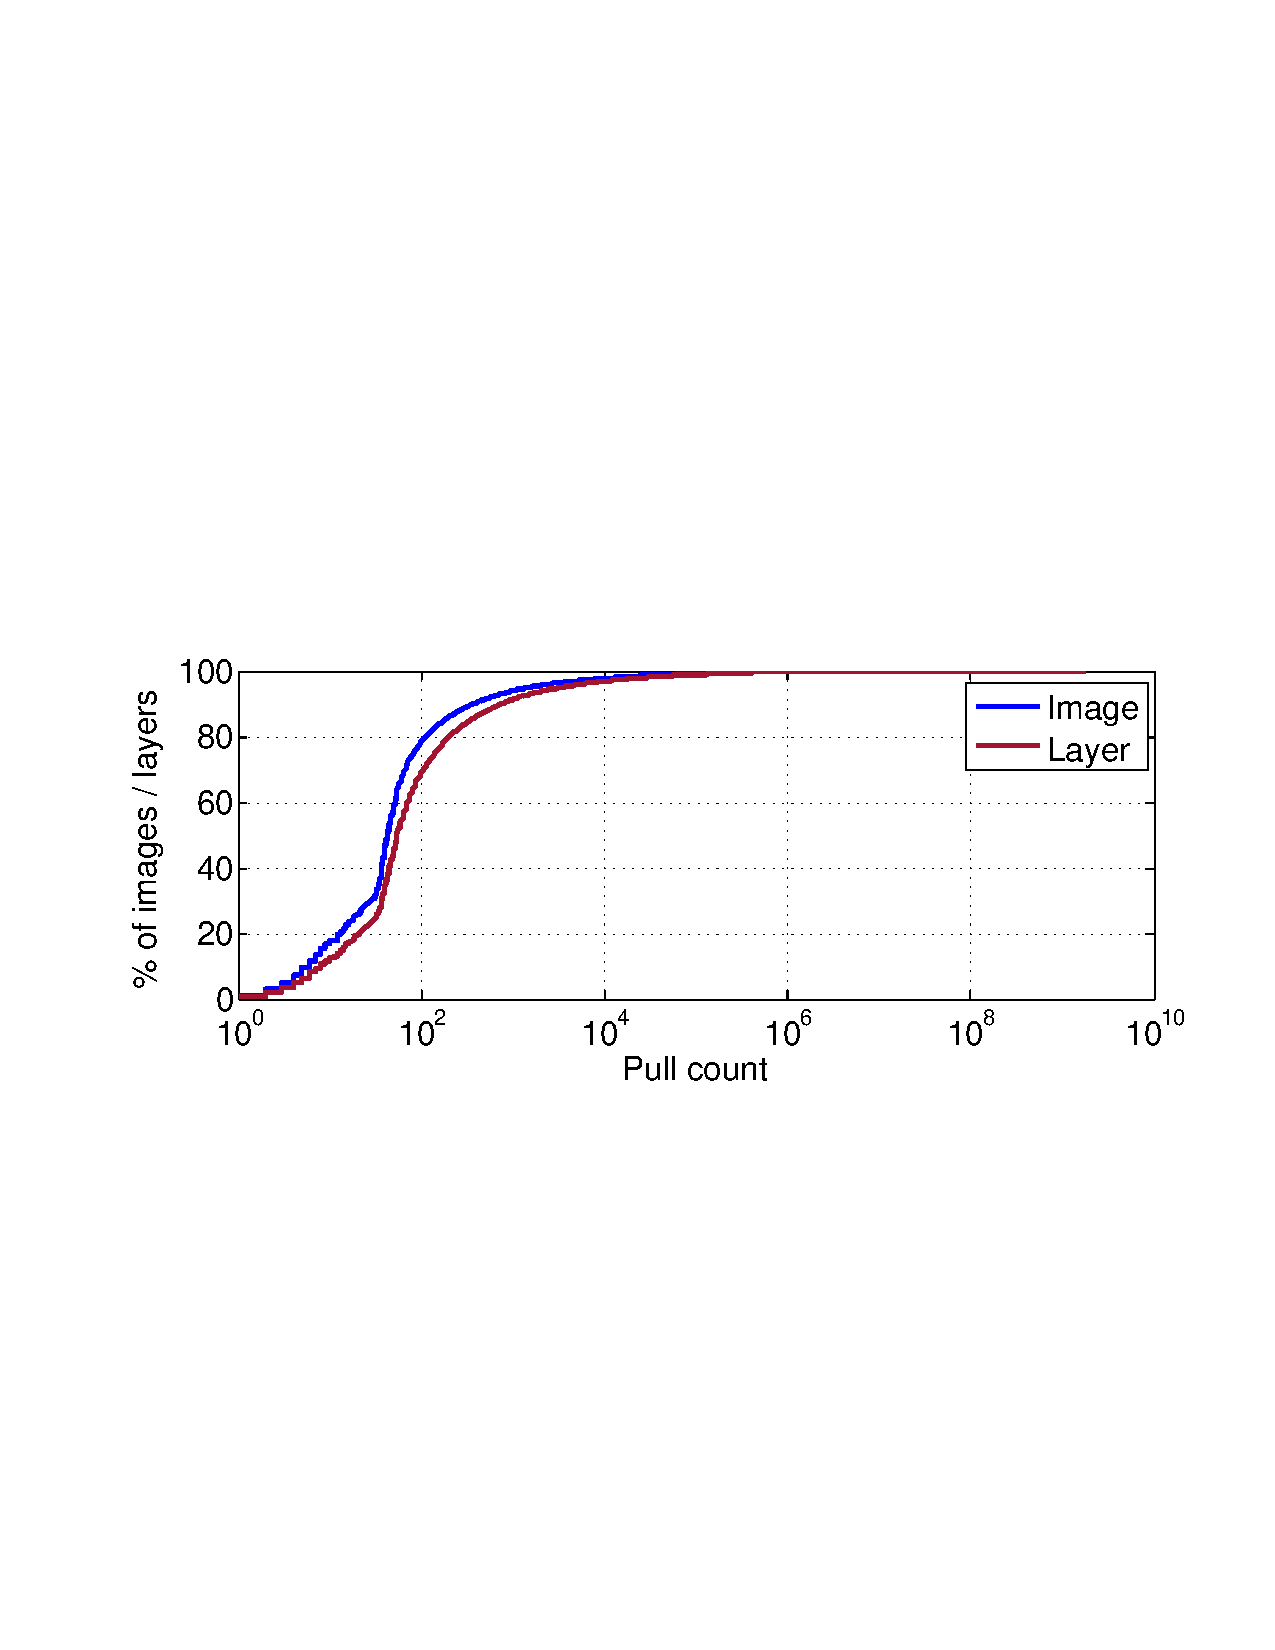
\includegraphics[width=0.4\textwidth]{graphs/pull-cnt.pdf}
	\caption{CDF of layer \& image pull count.
	}
	\label{fig:pull-cnt}
\end{figure}

\paragraph{Caching hot layers}
To reduce overhead, we suggest caching the hot/recently requested layers as
gzip compressed tar files. 
%
We observed that only a small proportion of images
and layers are frequently requested. 
%
A majority of images and layers are
\textit{cold}. 
%
As shown in Figure~\ref{fig:pull-cnt}, x-axis shows the total
number of pulls since the layers/images are stored in Docker Hub to May 30,
2017. 
%
We see that only 20\% and 10\% of images are pulled more that 100 and
360 times respectively. 
%
Similarly, only 20\% and 10\% of layers are pulled more
that 217 and 660 times. 
%
Note that the layers'pull count shown in
Figure~\ref{fig:pull-cnt} is calculated by aggregating all the images'pull
counts that refers this layer. 
%
Note that the image pull counts are crawled from
Docker Hub website. 
%
Actual layer pull count should be less than the number
shown in Figure~\ref{fig:pull-cnt} because pulling a image does not necessarily
pull all its containing layers as we don't pull the layers if they have already
been downloaded.


\subsection{Performance analysis}
%
\begin{figure}
	\centering
	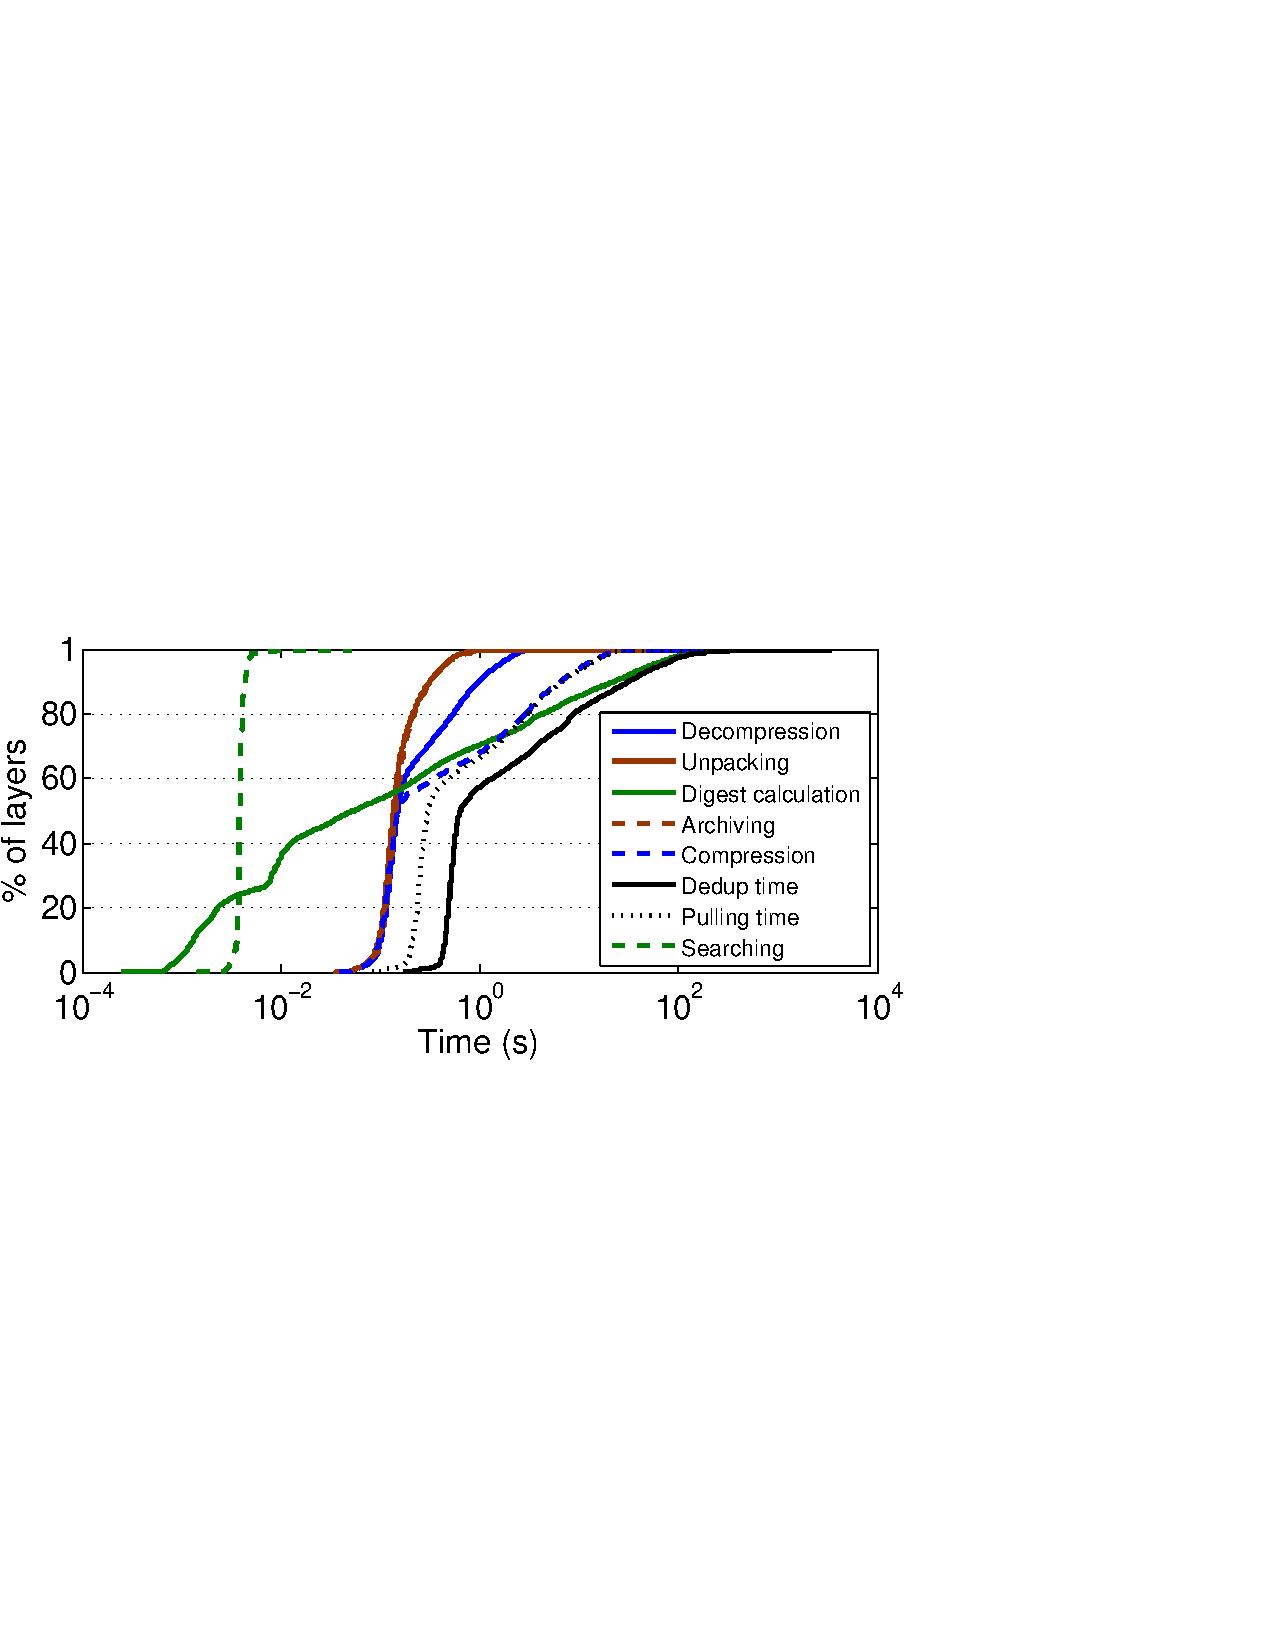
\includegraphics[width=0.48\textwidth]{graphs/res-time.pdf}
	\caption{Off-line file-level deduplication run time.
	}
	\label{fig:dedup-res}
\end{figure}

%\paragraph{Image \&. layer popularity skewness} 
%
% since dedup process only starts periodically when the
%workload is lower and only cold layers are evolved in dedup process (discussed
%in Section~\ref{subsec:FLCAS}).
%
%\lrcomment{By latency, do you mean the time it takes to perform the dedup? I
%wouldn't call that latency but rather run time or completion time.}
%
%\lrcomment{What exactly was the setup? Where those 60 requests submitted while
%the dedup was running and where they submitted only once or repeatedly?}

We wrote around 600 lines of Python code to perform file-level deduplication
operations on the layer dataset, specially, we read a layer from layer dataset
to a RAM disk (i.e., tmpfs) and then decompresses it. 
%
Then we
calculate each containing files' digests and append the layer-to-file digest
mapping records to a mapping table. 
%
Only unique files are maintained in RAM
disk while the redundant copies are removed.

To quantify the run time to perform file-level deduplication, we setup a
one-node Docker registry with 64~GB RAM and 32 Cores.  
%
We performed
deduplication of 60 concurrent layers for 0.9 Million layers in total.
%To improve searching performance, the
%mapping table is stored in Hive database~\cite{xxx}. 
%
%\lrcomment{Why are we using Hive for this? It seems overkill to me, especially
%for such small data. Even at scale, a KeyValue store would probably provide
%better performance than clunky MapReduce-based DB.}
%
Note that the pushing latency is not influenced by the file-level deduplication
because once the layer reaches registry, an response message will be sent to
the user. 
%
No addition delay will be added to the pushing time. 
%
However,
compression time will impact pulling latency since the files need to be packed
and compressed first and then sent to the users once registry receives pulling
requests to the cold layers. 
%
Similar to deduplication, to generate pull layer
requests, we randomly request 60 different layers in pralallel for 0.9 Million
layers. 
%
For pull layer requests, we packs and compresses the layer's containing
files by searching the mapping table for the layer digest. 

\paragraph{File-level deduplication run time}

%and pulling requests for  
%
Figure~\ref{fig:dedup-res} shows the breakdown of run time for each
involved operation: decompression time, unpacking time, file content digest
calculation time, and searching time.

First, among all the operations, we see that searching time is the
smallest. 
%
80\% of searching time is less than 0.004 s. 
%
The mapping table
maintains 0.98 million layer-to-file digest mapping records. 
%
Consider that more
than 1.7 million layers are stored in Docker hub and the number is still
increasing, it's better to choose a fast distributed database to provide high
searching performance and scalability.
%
%\lrcomment{How does our DB schema look and what are the search queries?}
  
Second, we see that digest calculation time spreads over a large range started
from 0.000005 s to 124.7 s. 
%
It's because digest calculation time largely
depends on the layer size. 
%
Typically, smaller layers contains a smaller number
of smaller files, which takes much less time to calculate their digests. 
%
While
if the layer is bigger, the digest calculation overhead will be higher. 
%
80\% of
digest calculation time is less than 4.21 s. 
%
Thus, we suggest that multiple-threading is needed to calculate the files'
digests simultaneously; 
%
Fast CPUs as well as more powerful computing nodes are
required to speed up digest calculation.

Third, the run time for decompression and unpacking have the same distribution
during the lowest response time range started from 0.04 s to 0.15 s. 
%
Around
60\% of decompression and unpacking time are less than 0.15 s. 
%
However,
decompression has the highest time than that of unpacking. 
%
80\% of
decompression is less than 0.55 s while 80\% of packing time is less than 0.21 s. 

Figure~\ref{fig:dedup-res} also shows the total time distribution for
file-level deduplication which is the sum of run time for decompression, unpacking,
digest calculation, and searching. 
%
We see that 80\% of file-level dedup time is
less than 9.09 s per layer.
%
%\lrcomment{Is that per layer or per file or per image?}
%
We also measured the throughput of 60 processes. 
%
Our one-node file-level
deduplication prototype can process about 3 layers/s. 
%
We suggest to use more
high powerful machines to improve throughput.

\paragraph{Pulling latency} Figure~\ref{fig:dedup-res} shows the pulling latency
distribution. 
%
Note that the pulling latency is the sum of archiving time,
compression time, and searching time and does not include network transfer
time. 
%
We can see that compression and archiving time almost share the same
distribution during the lowest response time range started from 0.04 s to 0.15
s. 60\% of compression and archiving time are less than 0.15 s.
%
While
compression has the highest run time. 
%
80\% of compression time is less than 2.82 s. 
%
We see that archiving time and compression contributes equally to pulling
latency when their run time are lower than 0.15 s while compression time almost
equals to pulling latency when the compression time is greater than 0.15 s. 
%
Hence, we
suggest that fast compression methods are required to reduce compression time.  
%
%\lrcomment{How does this compare to pulling without dedup? What's the overhead
%added?}


%
%\vcomment{What are the units for  $\sigma_{wl}$ and  $\sigma_{su}$?}
%
%\lrcomment{Do you mean it only runs through low workload periods? How are we
%predicting those or are we relying on some workload patterns? We should make
%that clear.}

%high while start file-level dedup \paragraph{FLCAS model}
%Figure~\ref{fig:file-dedup-model} shows an example of FLCAS.
%
%\vcomment{An example?..}
%
%\lrcomment{This explanation should come before the caching and light workloads
%paragraphs.}
%

%\paragraph{Caching hot layers to improve performance}
%\label{subsec:FLCAS}
%
%\begin{figure}
%	\centering
%	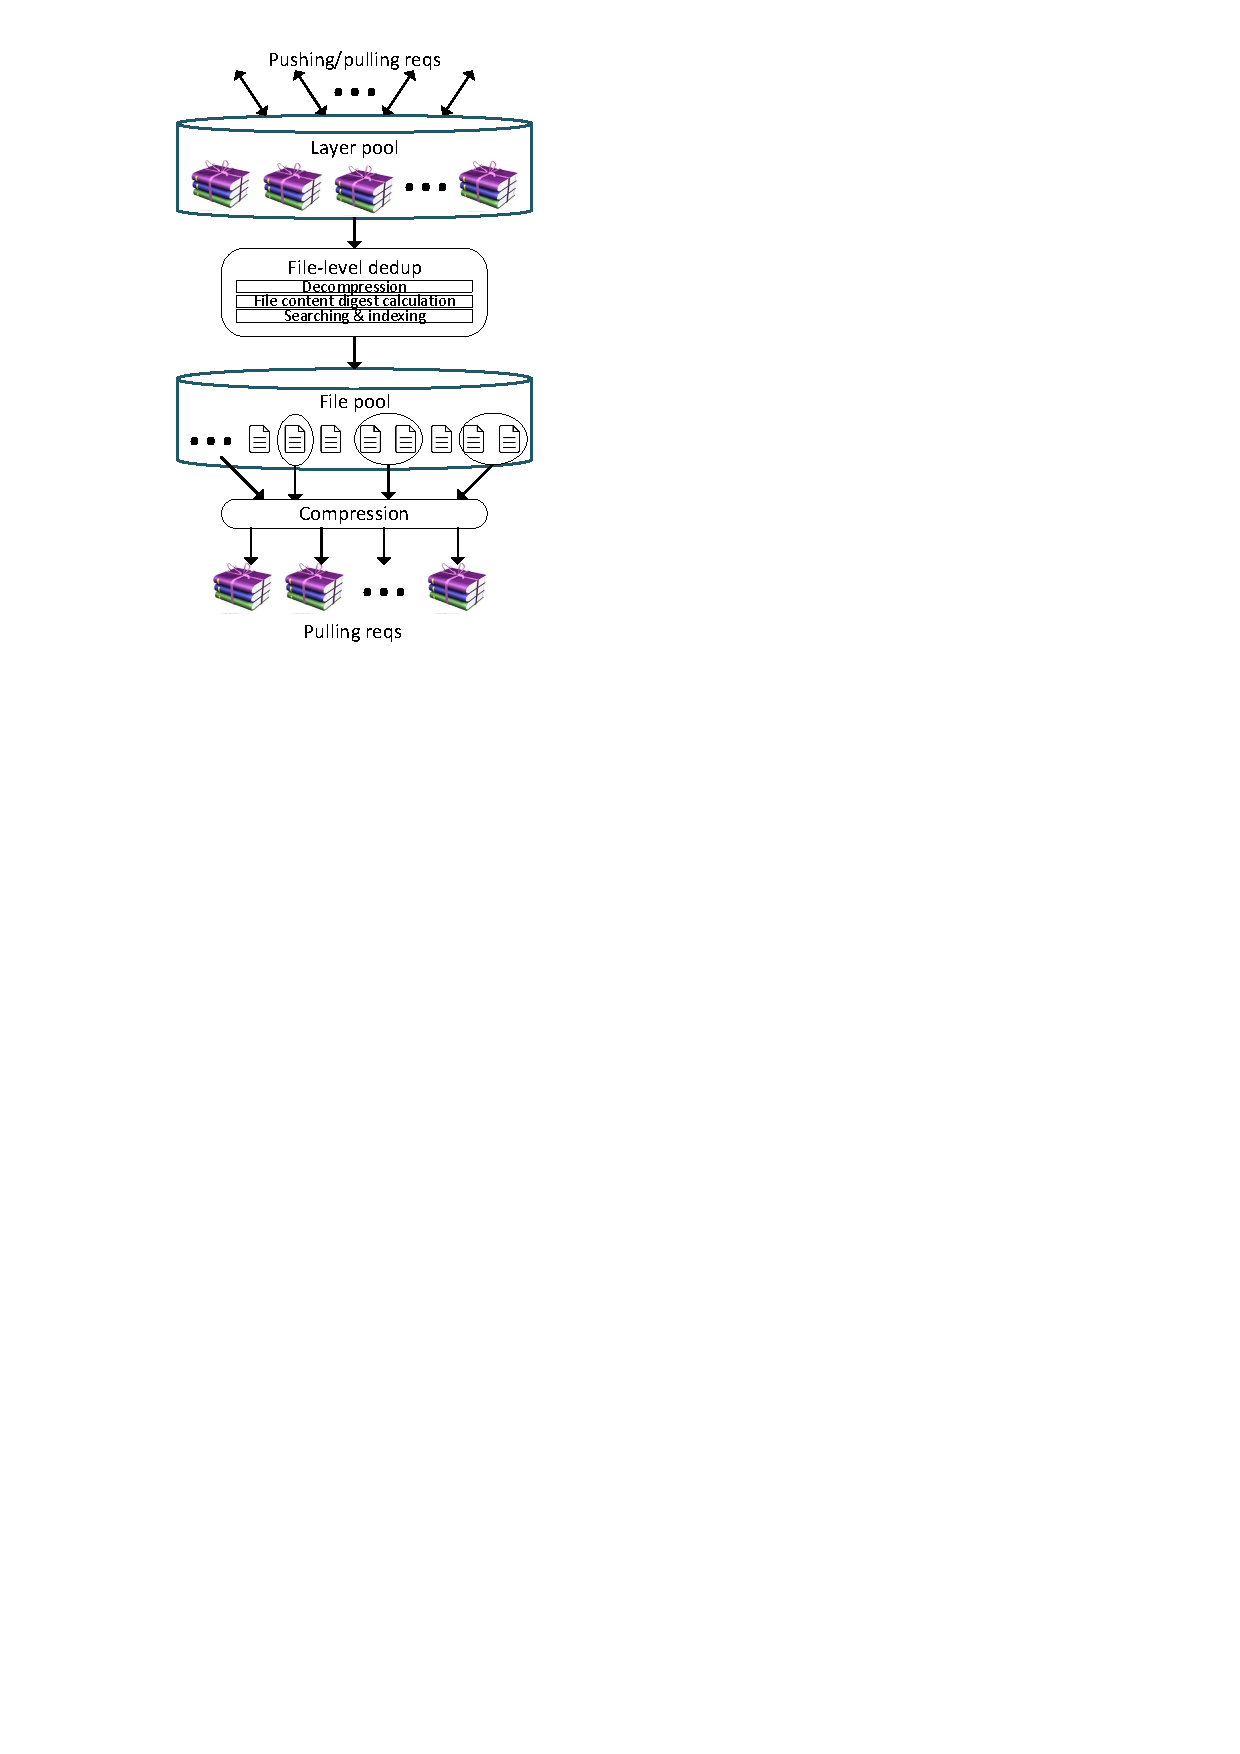
\includegraphics[width=0.3\textwidth]{graphs/graph_compression_layers.pdf}
%	\caption{File-level content addressable model.
%	\vcomment{1) Do not see ``cache'' word on the figure. 2) Font is too small in the middle section. 3) We need to describe how we depict layers vs. files. 4) There are pull requests both from the top and the bottom . I think we should just remove the part below the File pool.}
%	}
%	\label{fig:file-dedup-model}
%\end{figure}

%
%\vcomment{Who is ``it''?}\nancomment{addressed}
%
%
%\vcomment{Who are ``they''? Avoid using ``it'' and ``they''. Use actual nouns instead.}
%
 %a digest generated by a cryptographic hash function (such as ) 
%
%\vcomment{Let's use ``deduplication'' instead of ``dedup'' everywhere (because
%the letter one is informal)}

%\subsection{Trade-off discussion}

%

%\vcomment{I think there are two reasons for the cache 1) reduce push latency
%and 2) reduce pull latency. The text above talks only about reducing pull
%latencies.  We also need to talk about pushes.  Furthermore, the current
%discussion of pull counts does not really justify read (pull) cache.  For the
%read (pull) cache to be efficient there should be many pulls that access the
%same layers. E.g., that XXX\% of pulls go to the few YYY popular layers.
%Can we say that?}
%%
%\vcomment{somewhere we will need to talk about eviction policy, how to
%size the caching layer, and, finally, what happens if the cache is full.}
% 

%\subsection{Using RAM to load \&. process layers}
%
%To improve performance, we use RAM to temporarily store \textit{small} layers
%and directly process them in RAM.  Specially, we first load small layers in a
%RAM disk and perform decompression, unpacking, file content digest calculation
%in RAM, and remove them from RAM after completion.   According to our findings
%that majority (87.3\%) of layers that are less than 50M as shown in
%Figure~\ref{fig:image-layer-size}. So majority of layers can be stored and
%processed in RAM to speed up file-level dedup. 
%%layers that are less than 50M are stored and processed in RAM while the rest
%%layers are stored and processed in SSDs.
%%
%\lrcomment{This should still be part of 7.1 as it explains the strategy and not
%the prototype/simulations.}
%%
%\lrcomment{How are small layers defined? Where is the threshold?}
%
%majority (xxx) of layers'dedup times are less than xxx.
%during peak workload, which means that we start file-level dedup whenever it receives a layer. 
%To simulate the high intensive workload, we first sent a sequential of layer pushing requests to registry and stored, then we measure the file-level dedup  
%, archiving time, and compression time.
%Second, compare the latency for each operation, we see that xxxx
%\paragraph{Latency breakdown}
%We calculated the latency for each operation for all layers as shown as Table~\ref{tbl:latency_breakdown}.
%Figure~\ref{xxx} shows the compression time across 

%\begin{figure}[!t]
%	\centering
%	\subfigure[CDF of repositories by pull count]{\label{fig_pull_cnt_total}
%		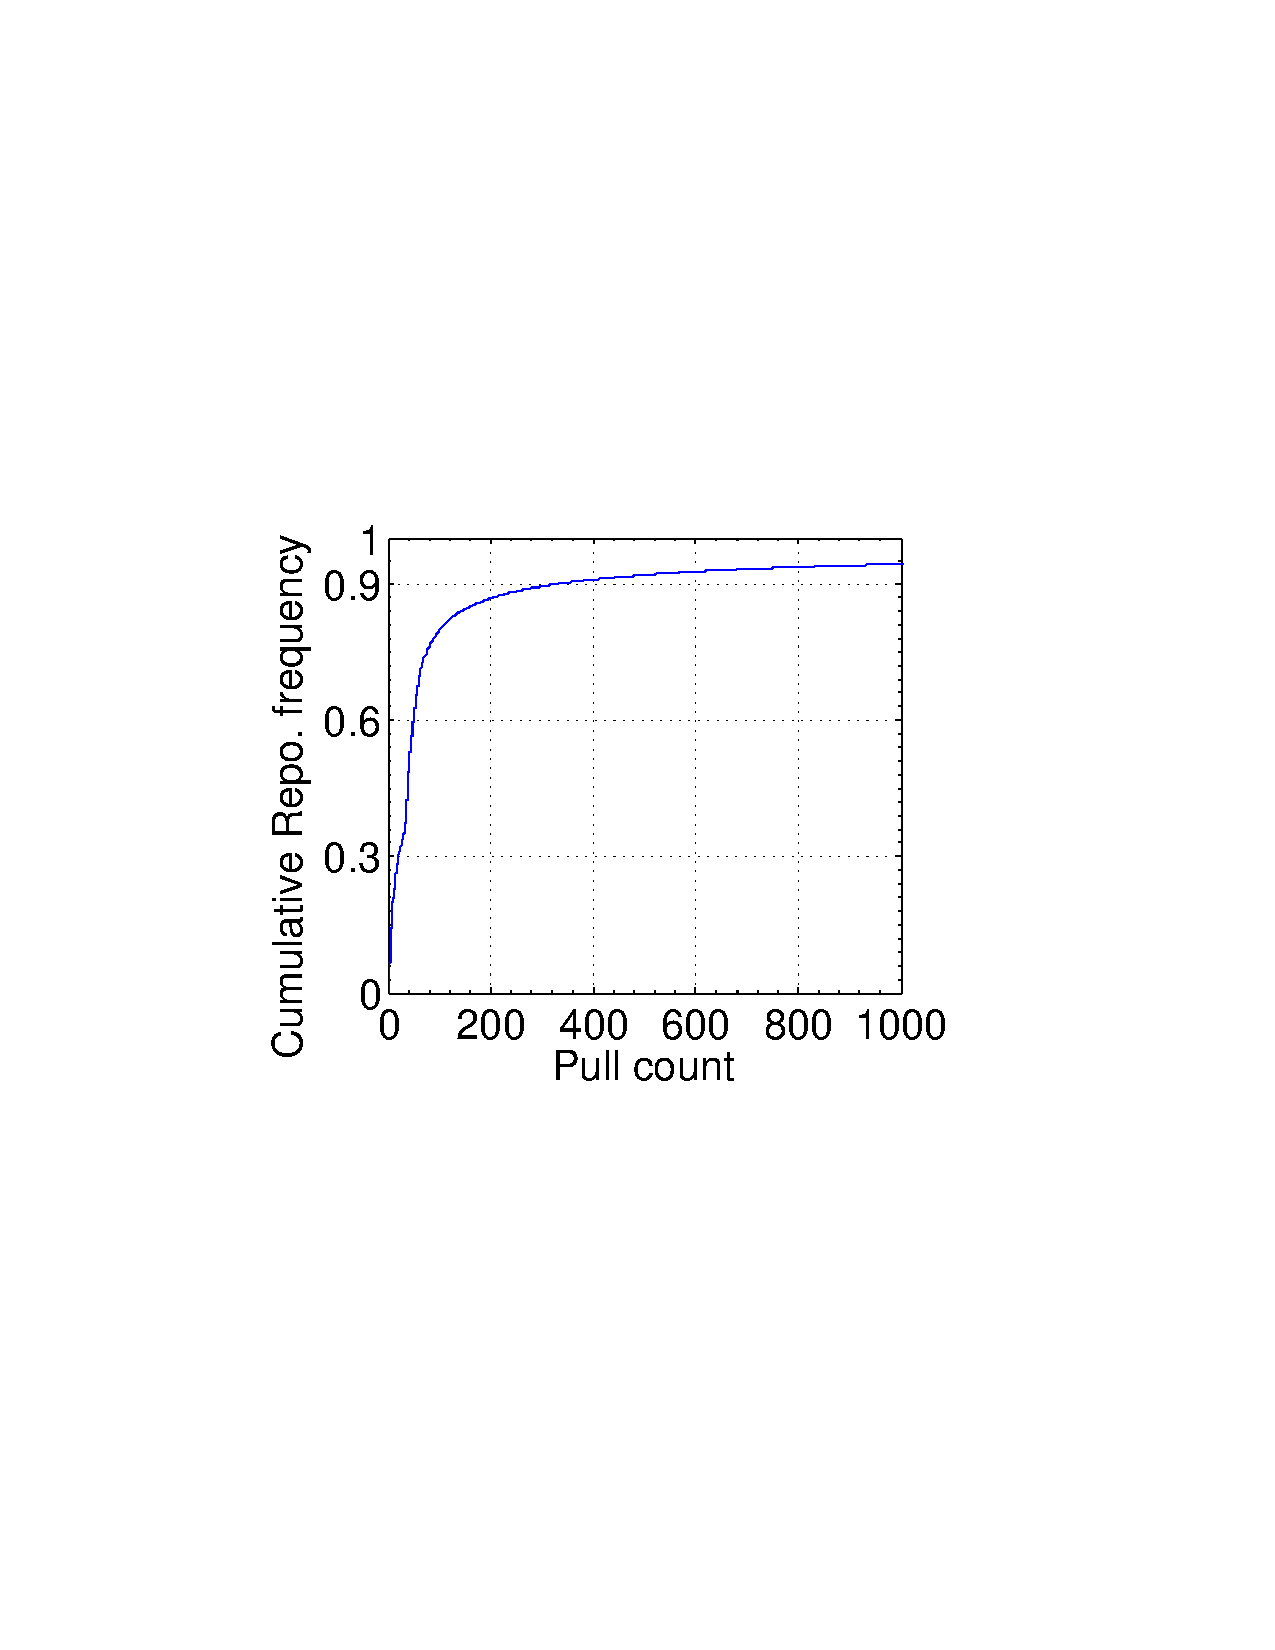
\includegraphics[width=0.23\textwidth]{graphs/pull_cnt.pdf}%
%	}
%	\subfigure[Histogram of repositories by pull count]{\label{fig_pull_cnt_count}
%		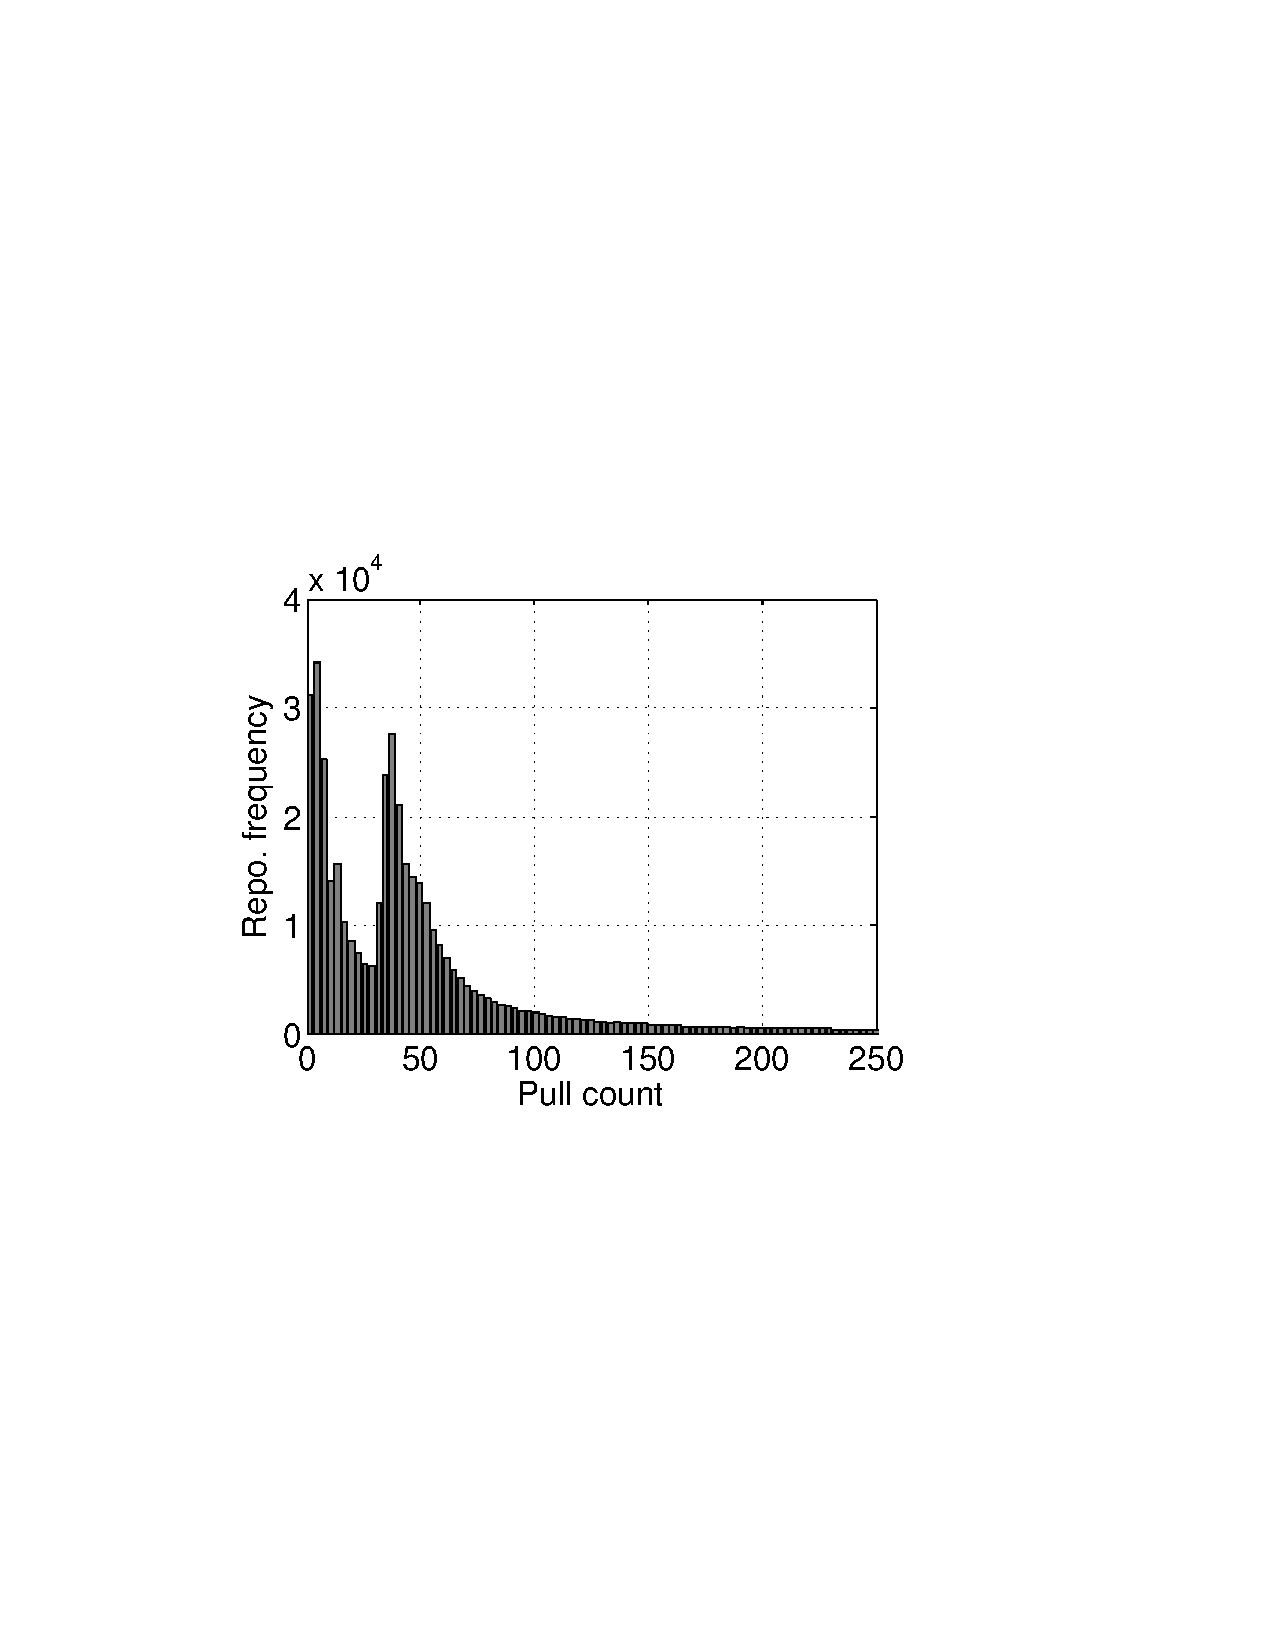
\includegraphics[width=0.22\textwidth]{graphs/count_pull_cnt.pdf}
%	}
%	\caption{Repository popularity distribution}
%	\label{fig-pop}
%\end{figure}

%=======================================
%|             OLD VERSION              |
%=======================================

%\paragraph{Latency distribution for each operation}
%\subsubsection{When to start file-level dedup?} 

%\paragraph{Latency distribution for each operation}

%\paragraph{Small compression ratio and small layer size}
%
%\begin{figure}[!t]
	\centering
	\subfigure[CDF of compression ratio]{\label{fig_cdf_compression_ratio}
		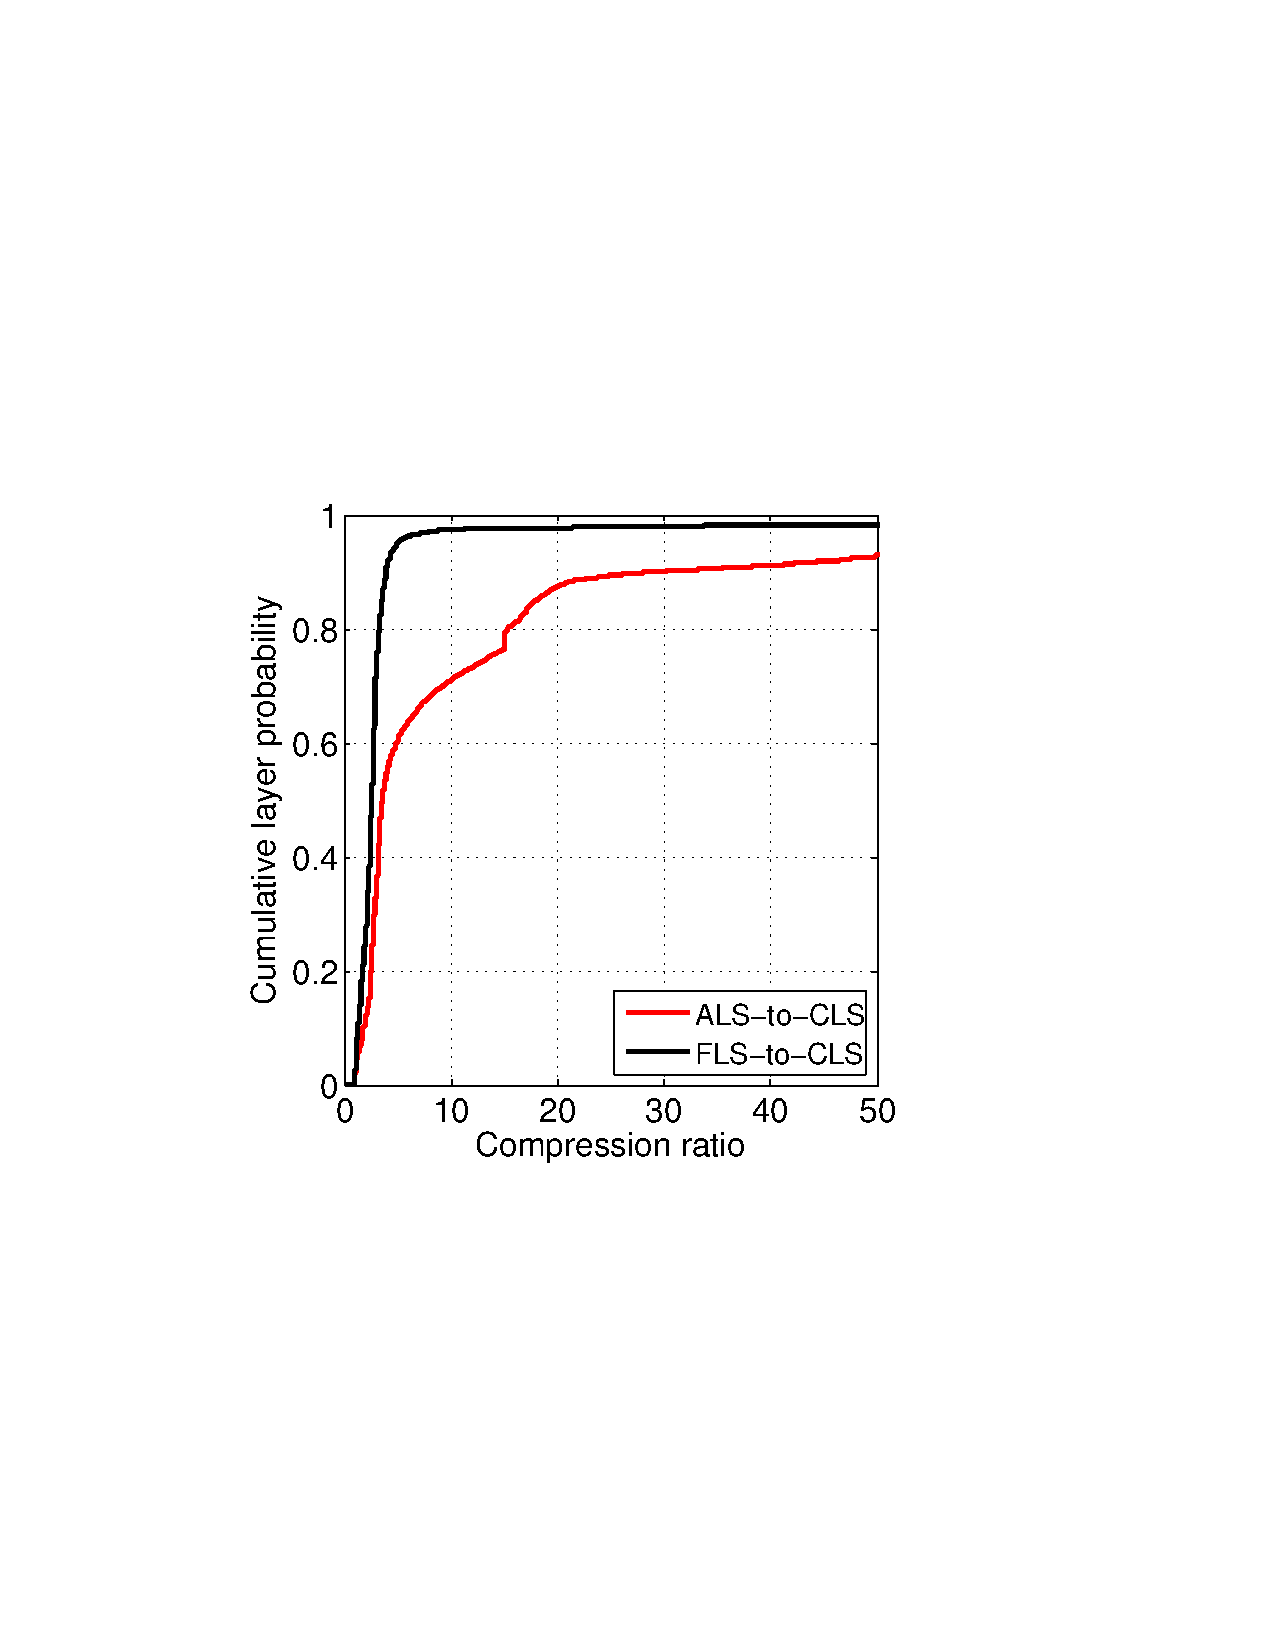
\includegraphics[width=0.23\textwidth]{graphs/cdf_compression_ratio.pdf}
	}
	\subfigure[Histogram of comp. ratios]{\label{fig_his_compression_ratio}
		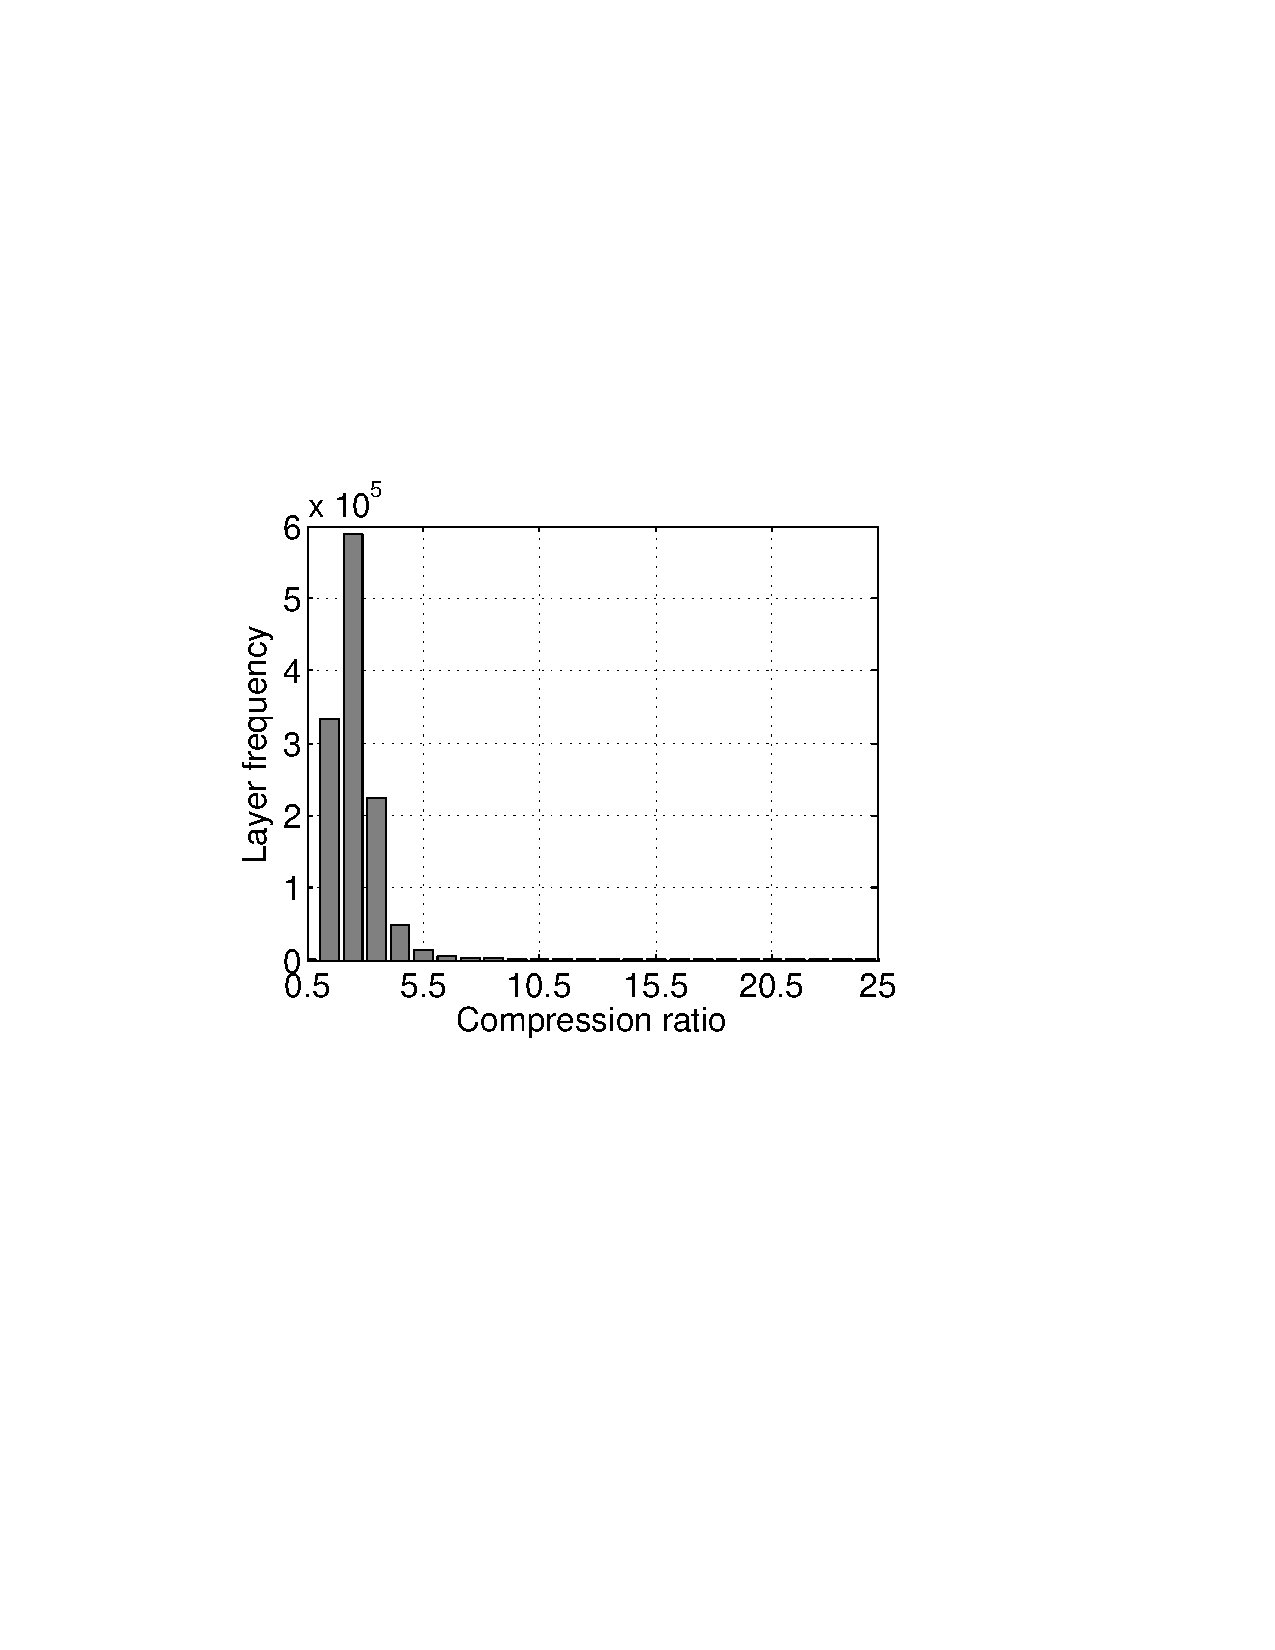
\includegraphics[width=0.223\textwidth]{graphs/his_compression_ratio.pdf}
	}
	\caption{Layer compression ratio distribution
	%\vcomment{Different colors are used in figure (a) and (b) FLS/CLS\nancomment{will address later}}
	}
	\label{fig-compression-ratio}
\end{figure}

%
%\begin{figure}[!t]
	\centering
	\subfigure[CDF of layer sizes]{\label{fig_layer_size_cdf}
		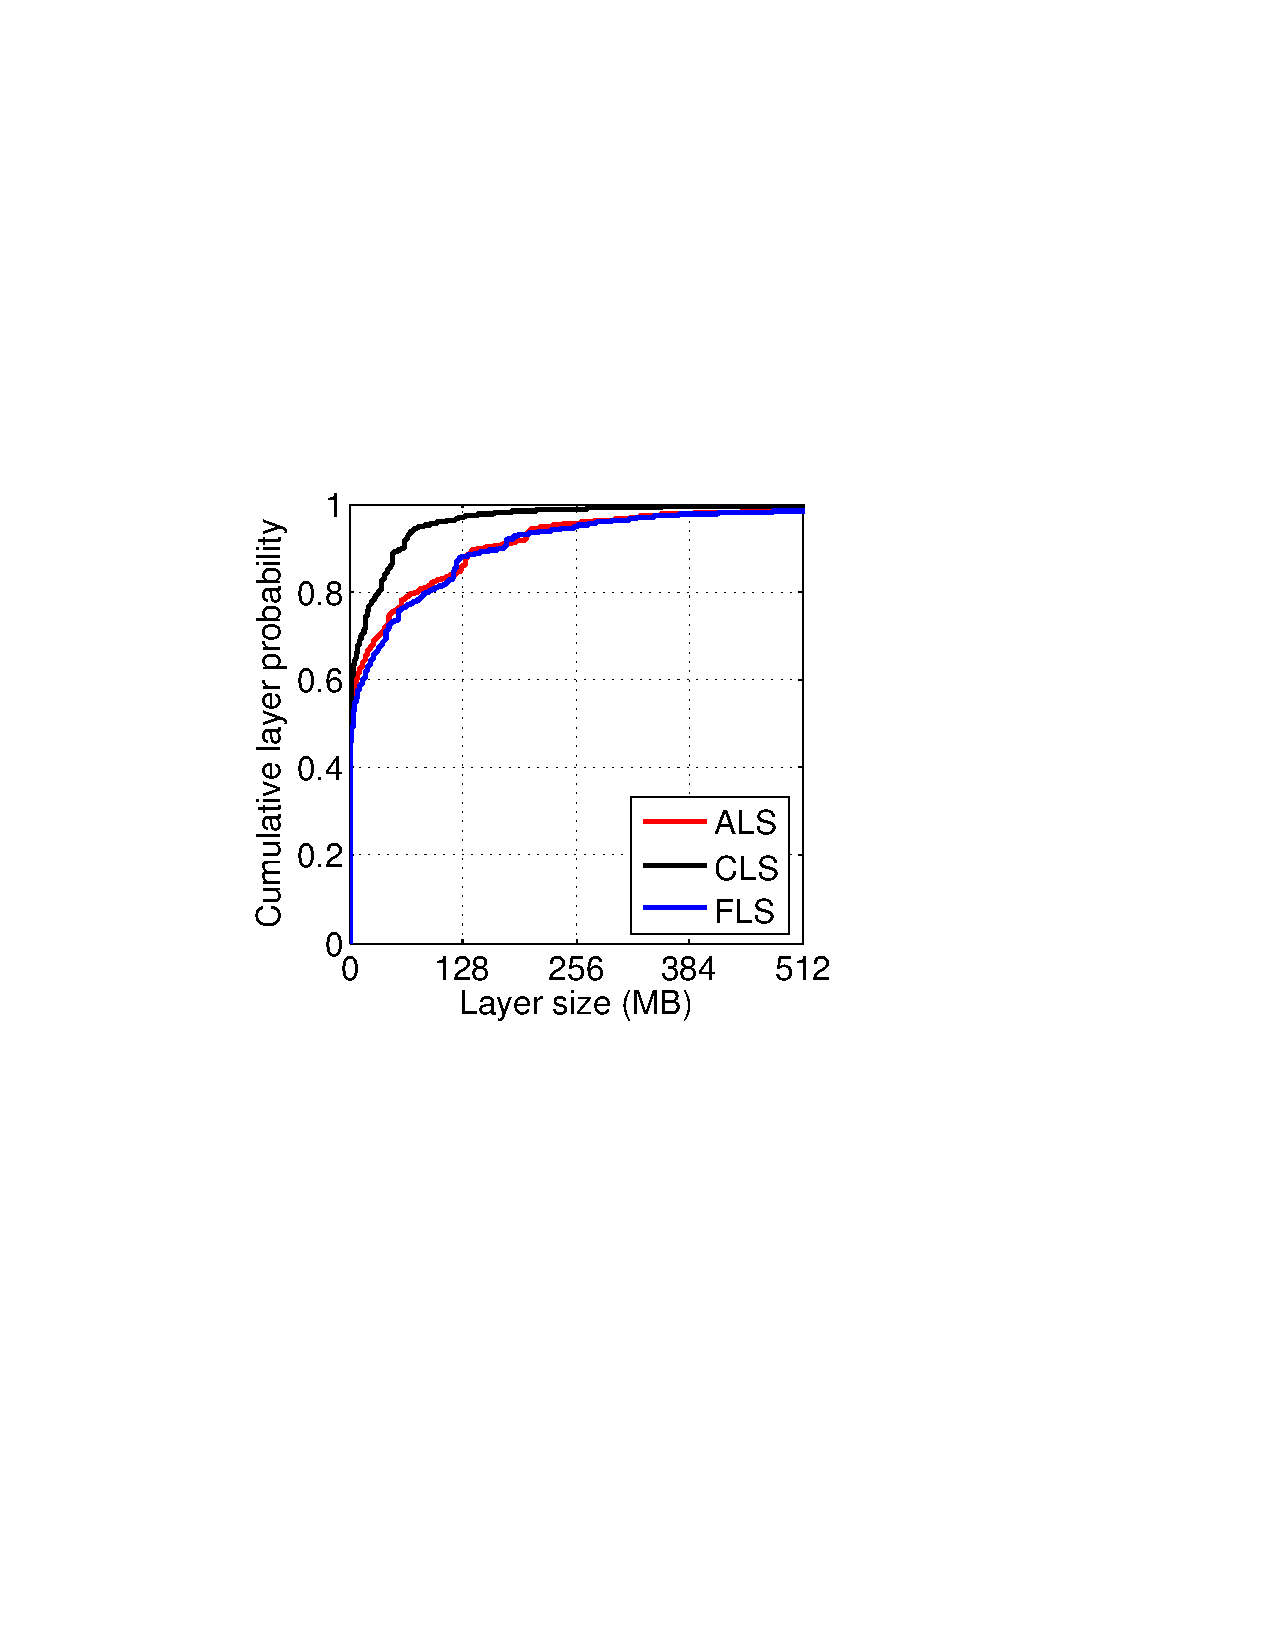
\includegraphics[width=0.234\textwidth]{graphs/layer_size_mb.pdf}
	}
	\subfigure[Histogram of layer sizes]{\label{fig_hist_layer_size}
		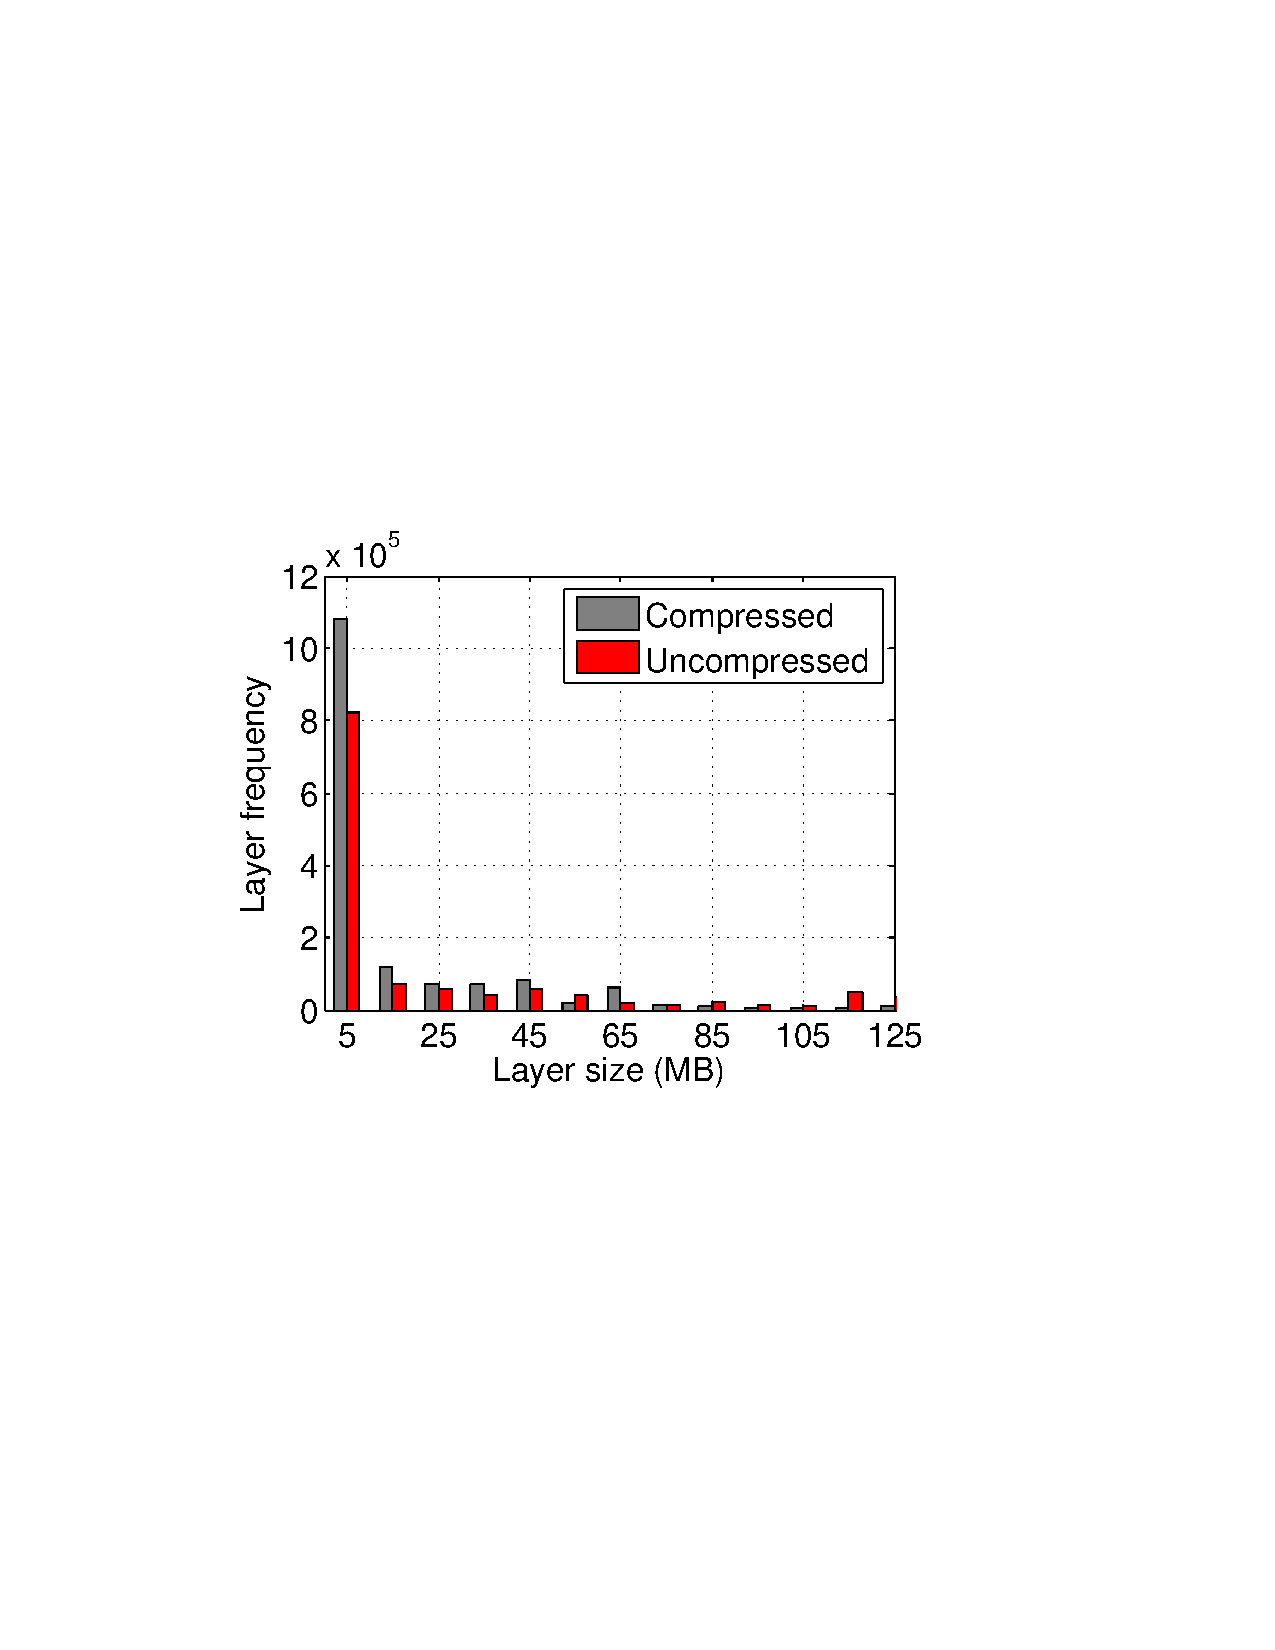
\includegraphics[width=0.213\textwidth]{graphs/hist_layer_size.pdf}
	}
	\caption{Layer size distribution
	\vcomment{Let's use CLS, ALS, and FLS abreviations\nancomment{addressed}}.
	\vcomment{CLS size should go first}.
	\vcomment{We need to use different types of lines (solid, dotted, etc.)
		or markers (round, triangular)}.
	\vcomment{In figure B it is not clear to which bar group corresponds
		  to which layer size. I suggest to try to rotate the graph
		  by 90 grads to fit all layer size labels.\nancomment{aligned label with bar}}
	}
	\label{fig-layer-size}
\end{figure}

%
%We found that most layers'compression ratio is really lower (?) while most of layers have a smaller size. 
%So how about we use archiving instead of compression if the network speed is higher (?GB/s)?

%\paragraph{Network transfer speed is high!}

%\subsubsection{File-level content addressable storage for cold layers}

%\begin{figure}
%	\centering
%	\includegraphics [width=0.45\textwidth]{plots/exp-total-stev-erase.eps}
%	\subfigure[]{\label{fig:per_layer_ratio_fcnt_cdf}
%		\includegraphics [width=0.23\textwidth]{graphs/}
%	}
%	\subfigure[Similar layer dedup]{\label{fig:per_layer_ratio_fcnt_pdf}
%		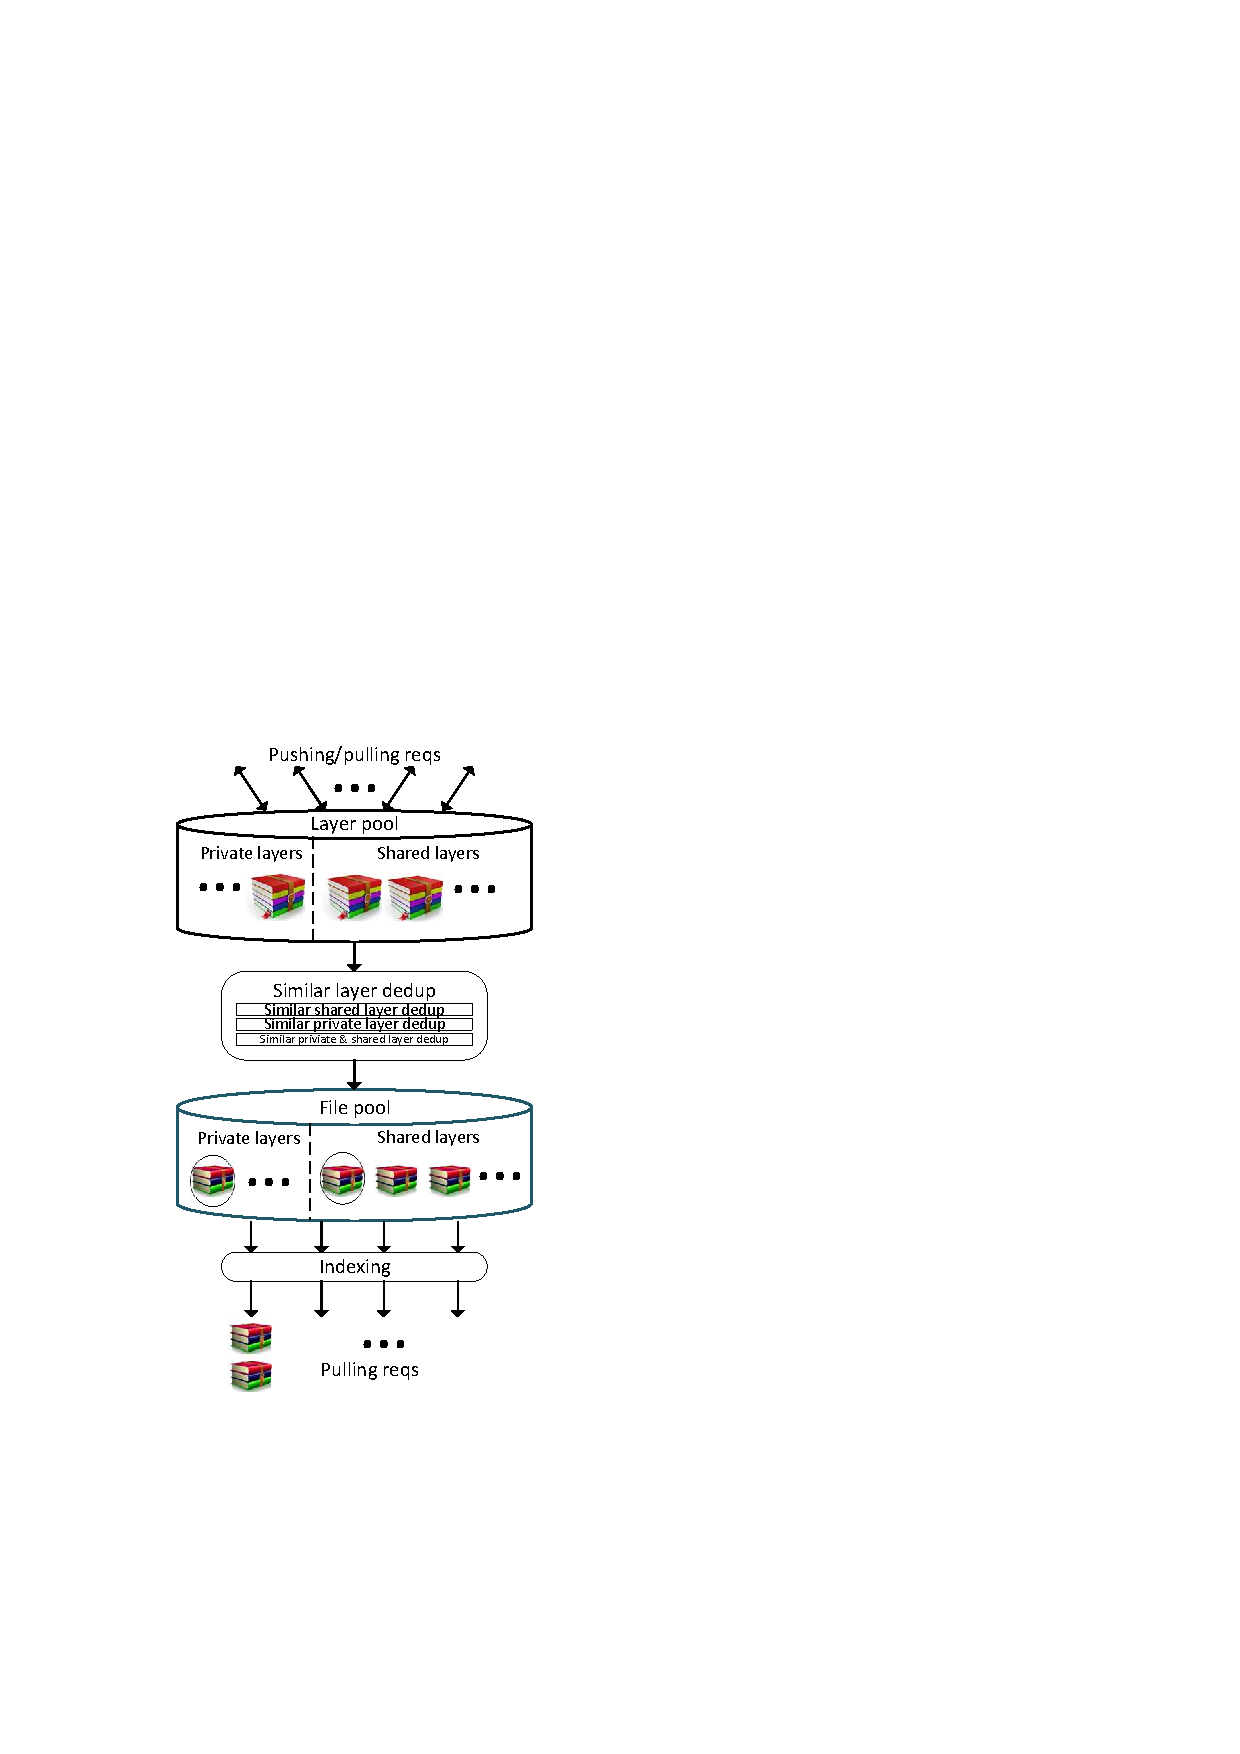
\includegraphics [width=0.22\textwidth]{graphs/graph_reconstruct_layers.pdf}
%	}
%	\caption{File-level content addressable storage model}
%	\label{fig:eval-stdev-erasure-cnt}
%\end{figure}

%\subsection{Hints for performance improvement and storage saving}

%\begin{table} 
%	\centering 
%	\scriptsize  
%	%\begin{minipage}{.5\linewidth}
%	\caption{Latency breakdown} \label{tbl:latency_breakdown} 
%	\begin{tabular}{|l|l|l|l|l|}%p{0.14\textwidth} 
%		\hline 
%		% after \\: \hline or \cline{col1-col2} \cline{col3-col4} ... 
%		% after \\: \hline or \cline{col1-col2} \cline{col3-col4} ... 
%		Operations/latency (S) & max & min & median & avg.\\
%		\hline
%		 gunzip decompression (RAM) & 257.16  & 0.04  & 0.15  & 0.39 \\
% 		\hline
% 		tar extraction (RAM) & 43.41  & 0.04  &  0.14  & 0.18 \\
%		\hline
%		Digest calculation (RAM) & 3455.01  & $<$0.00  & 0.05 & 10.65 \\
%		\hline
%		tar archiving (RAM)  & 53.44 & 0.04 & 0.14 & 0.19\\
%		\hline
%		gzip compression (RAM) & 496.04 & 0.04 & 0.15 & 2.10 \\
%%		\hline
%%		Total time (RAM) (with compression) & & & & \\
%%		\hline
%%		Total time (RAM) (without compression) & & & & \\
%		\hline
% 		\hline
% 		gunzip decompression (SSD) &   &   &    &  \\
% 		\hline
% 		tar extraction (SSD) &   &   &    &  \\
%		\hline
%		Digest calculation (SSD) &  &  & & \\
%		\hline
%		tar archiving (SSD) &  &  & & \\
%		\hline
%		gzip compression (SSD) & &  &  & \\
%%		\hline		 
%%		Total time (SSD) (with compression) & & & & \\
%%		\hline
%%		Total time (SSD) (without compression) & & & & \\
%		\hline
%		\hline
%		Network transfer & 20587.94 & $<$ 0.00 & $<$ 0.00 & 1.20 \\
%		\hline 	
%	\end{tabular} 
%\end{table}


%\begin{table} 
%	\centering 
%	\scriptsize  
%	%\begin{minipage}{.5\linewidth}
%	\caption{Summary of layer \& image characterization} \label{tbl:redundant_ratio} 
%	\begin{tabular}{|l|l|l|l|l|}%p{0.14\textwidth} 
%		\hline 
%		% after \\: \hline or \cline{col1-col2} \cline{col3-col4} ... 
%		% after \\: \hline or \cline{col1-col2} \cline{col3-col4} ... 
%		Metrics & max & min & median & avg.\\
%		\hline
%		Compressed layer size &   &   &   &  \\
%		\hline
%		Uncompressed layer size &   &   &    &  \\
%		\hline
%		Archival size &  &  & & \\
%		\hline
%		Compression ratio &   &   &    &  \\
%		\hline
%		Layer pull cnt. &  &  & & \\
%		\hline
%		File cnt. per layer &  &  & & \\
%		\hline
%		Dir. cnt. per layer &  &  & & \\
%		\hline
%		Layer depth &  &  & & \\
%		\hline
%		\hline
%		Compressed image size &  &  & & \\
%		\hline
%		Uncompressed image size & &  &  & \\
%		\hline
%		Archival image size & &  &  & \\
%		\hline
%		Compression ratio &   &   &    &  \\
%		\hline
%		Image pull cnt.  &  &  & & \\
%		\hline
%		Layer cnt. per image  &  &  & & \\
%		\hline
%		Shared layer cnt. per image  &  &  & & \\
%		\hline
%		File cnt. per layer &  &  & & \\
%		\hline
%		Dir. cnt. per layer &  &  & & \\
%		\hline	
%	\end{tabular} 
%\end{table} 

%\subsection{Constructing shared layers for redundant directories/files}
%
%\paragraph{Smaller number of layers are shared among different images}
%\begin{figure}[!t]
	\centering
	\subfigure[CDF of layer reference count]{\label{fig_repeate_layer}
		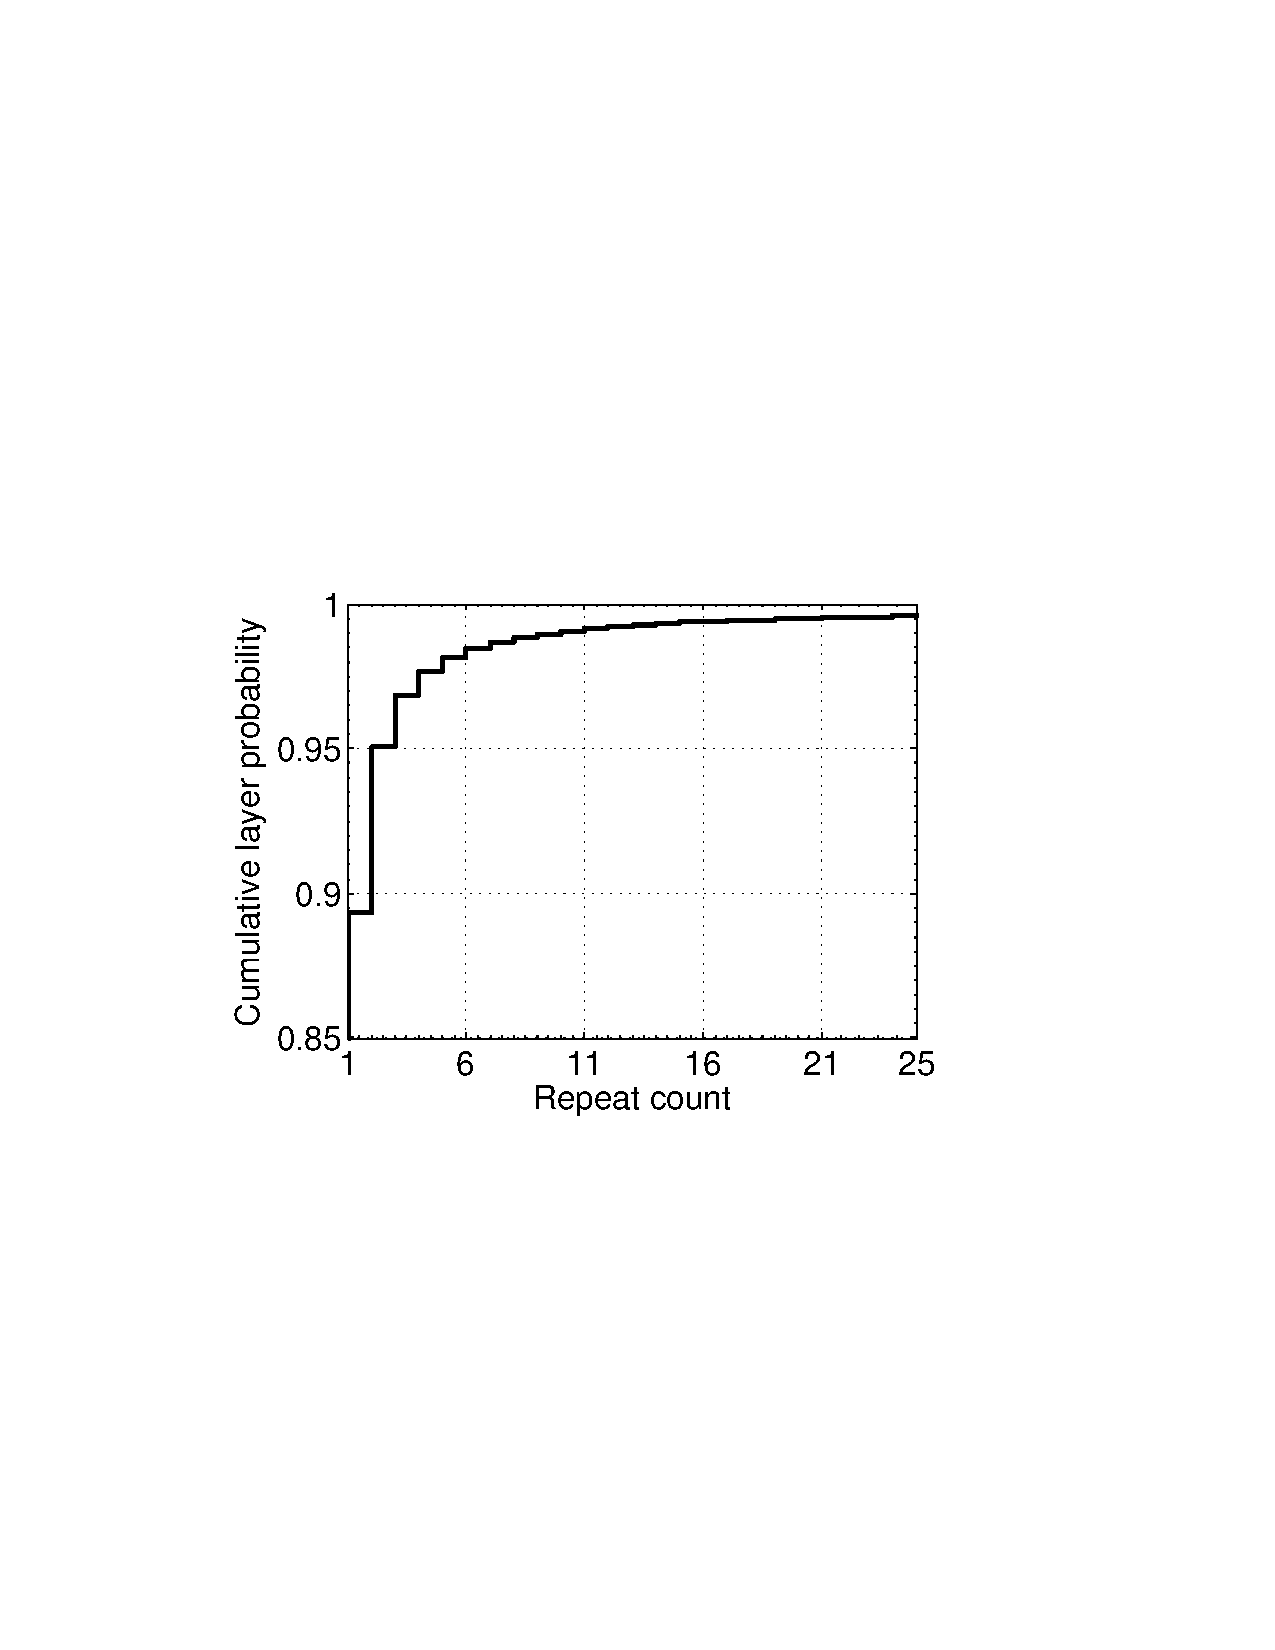
\includegraphics[width=0.23\textwidth]{graphs/repeate_layer.pdf}
	}
	\subfigure[Histogram of layer reference count]{\label{fig_hist_repeate_layer}
		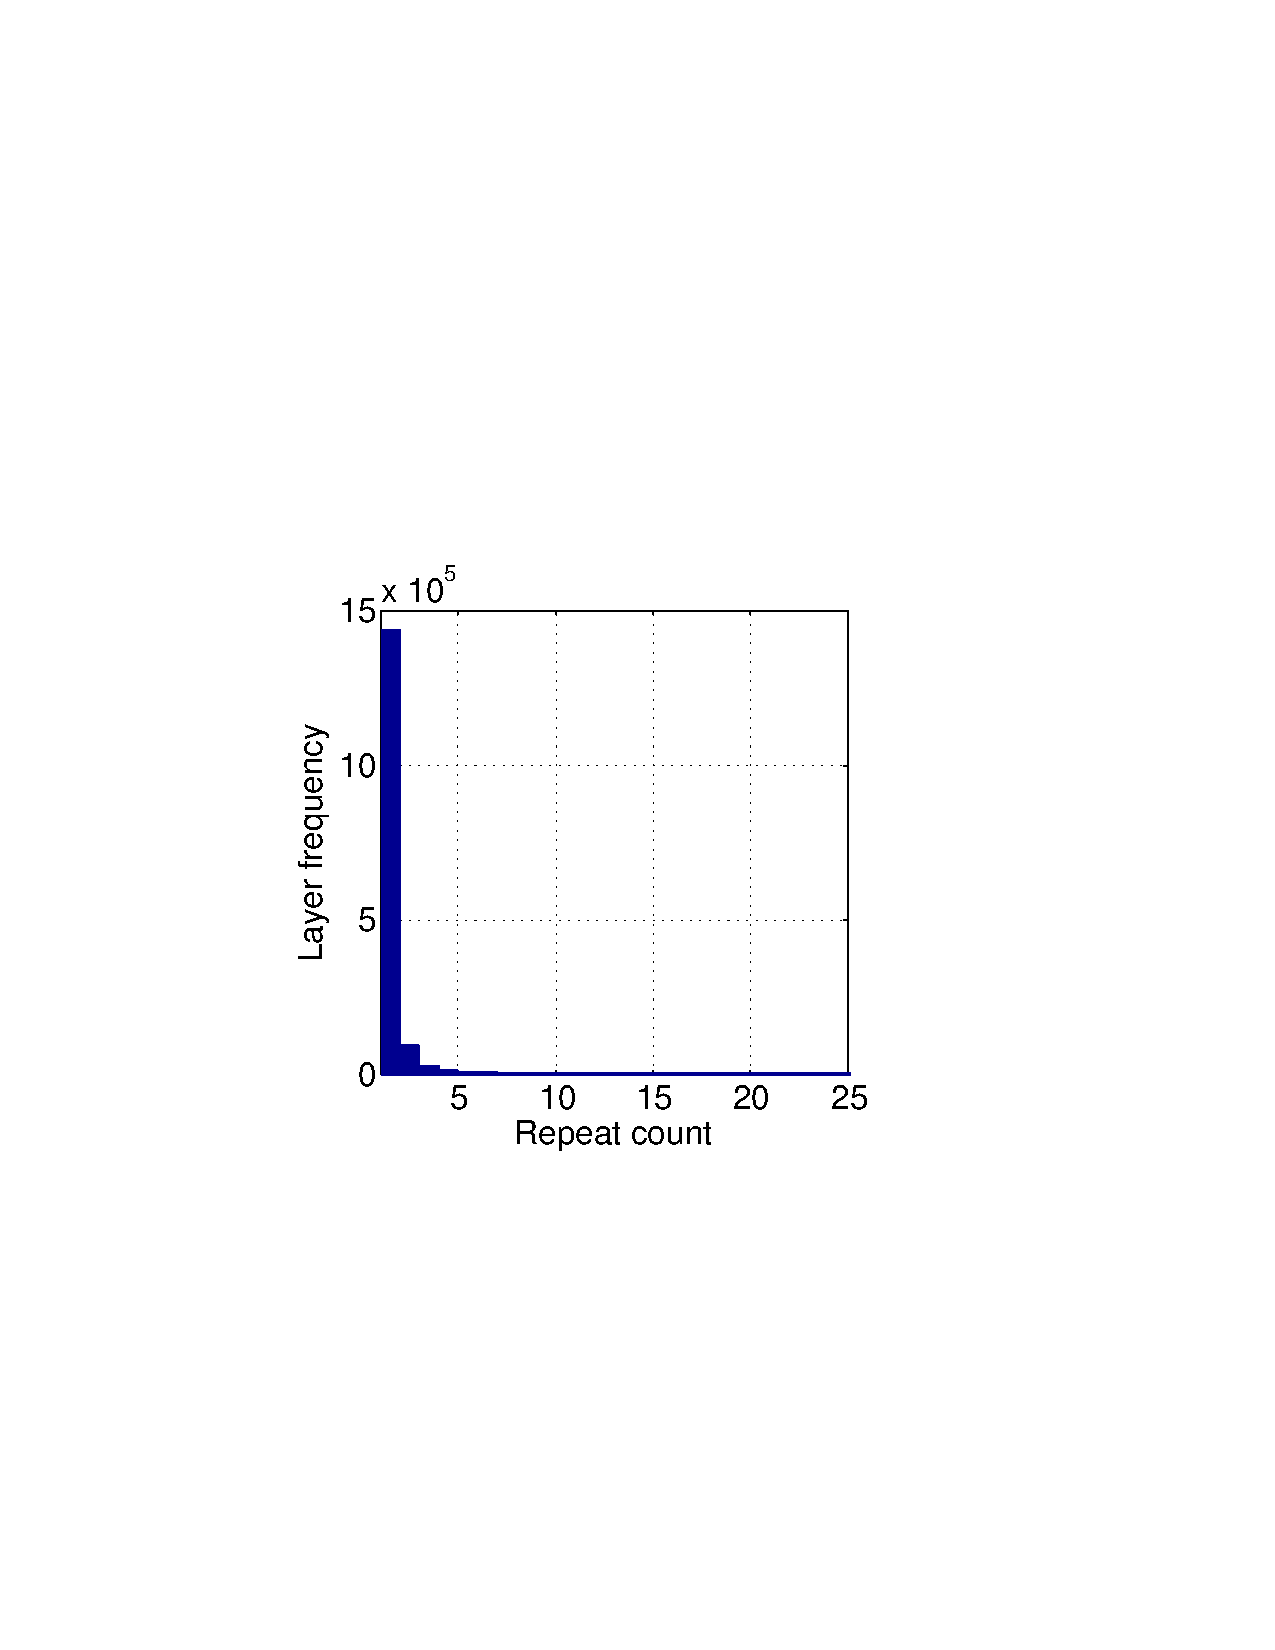
\includegraphics[width=0.223\textwidth]{graphs/hist_repeate_layer.pdf}
	}
	\caption{Layer reference counts across all images}
	\label{fig-repeat-layer-cnt}
\end{figure}
%
%\paragraph{Smaller pull latency than recompression model} the registry can prepare the reconstructed layers before users issue a pull request. But this model requires users to rebuild two layers.

%\subsubsection{Summary of Suggestions/trade-offs between dedup ratio and recompression overhead}
%
%\paragraph{1. using archiving instead of compression}
%\paragraph{2. using file-level dedup for cold images/layers}
%\paragraph{3. using file-level dedup economically}
%When to trigger file-level dedup?
%\paragraph{4. constructing shared layers for redundant dirs/files, for example,}
%%\subsection{Layer reconstruction model}
%%\subsubsection{Reconstruction overhead}
%%\subsubsection{Trade-offs between dedup ratio and reconstruction overhead}
%%\paragraph{Dedup ratio VS. Rebuild overhead}
%%\subsection{Evaluation results}
